%!TEX root=../GaugeCNNTheory.tex

\section{مدل اسباب‌بازی: کانولوشن‌های موبیوس هم‌متغیر انعکاس}
\label{sec:mobius_conv}

برای ملموس‌تر کردن ملاحظات نظری بخش‌های قبلی، اکنون به یک نمونه کاربرد می‌پردازیم.
در حالی که از اهمیت عملی فوری برخوردار نیست، کانولوشن‌های $\GM$ روی نوار موبیوس یک مدل اسباب‌بازی مناسب هستند زیرا هندسه آن و نظریه نمایش درگیر به‌ویژه ساده است.
به دلیل غیرجهت‌پذیر بودن آن، چارچوب‌های مرجع فقط می‌توانند (به‌طور هموار) تا حد انعکاس‌ها ترجیح داده شوند.
همانطور که انتظار می‌رود، \CNN های مستقل از مختصات، با اعمال توابع الگوی هم‌متغیر انعکاس، از پیاده‌سازی ساده‌لوحانه وابسته به مختصات بهتر عمل می‌کنند.
علاوه بر این نشان داده می‌شود که آنها تحت عمل گروه ایزومتری نوار موبیوس هم‌متغیر هستند.

\etocsettocdepth{3}
\etocsettocstyle{}{} % from now on only local tocs
\localtableofcontents

بخش~\ref{sec:mobius_geometry} در ادامه هندسه نوار موبیوس مسطح را مورد بحث قرار می‌دهد.
به دلیل پیچ آن، گروه ساختار آن نمی‌تواند بیش از گروه انعکاس~$G=\Flip$ کاهش یابد، به‌طوری که باید اطلس $\Flip$ از گیج‌ها را همانطور که در شکل~\ref{fig:mobius_conv_gauges} نمایش داده شده، در نظر گرفت.
گروه ایزومتری توسط چرخش‌ها در امتداد نوار داده می‌شود و تبدیل‌های گیج با مقادیر $\Flip$ را القا می‌کند.
میدان‌های ویژگی مستقل از مختصات $\RM$، که برخی از آنها در بخش~\ref{sec:mobius_representations} معرفی می‌شوند، لزوماً باید مطابق با نمایشی از گروه انعکاس تبدیل شوند.
بخش~\ref{sec:mobius_cnn_ops_analytical} عملیات شبکه کانولوشنی مستقل از جهت‌گیری را مورد بحث قرار می‌دهد.
این به‌ویژه مفهوم کرنل‌های $G$-راهبری‌پذیر را روشن می‌کند اما همچنین بایاس‌های هم‌متغیر انعکاس و غیرخطی‌ها را پوشش می‌دهد.
پیاده‌سازی عددی خانواده مدل پیشنهادی در بخش~\ref{sec:mobius_experiment_main} مورد بحث و ارزیابی قرار می‌گیرد.
کد به‌طور عمومی در \url{https://github.com/mauriceweiler/MobiusCNNs} در دسترس است.


%!TEX root=../GaugeCNNTheory.tex

\subsection{هندسه نوار موبیوس}
\label{sec:mobius_geometry}

منیفلد $M$ مورد بررسی نوار موبیوس مسطح با مرز است همانطور که در شکل~\ref{fig:weight_sharing_ambiguity} (راست) نشان داده شده است.
می‌توان آن را به‌عنوان ساخته شده از زیرمجموعه مستطیلی $[0,X] \times [0,Y]$ از $\R^2$ و چسباندن دو انتهای مقابل به‌شکل پیچ‌خورده در نظر گرفت.
با این تعریف، نوار موبیوس متریک کانونی $\R^2$ را به ارث می‌برد که آن را با ساختار ریمانی مجهز می‌کند.
متریک به‌ویژه اتصال لوی-چیویتا و در نتیجه نگاشت‌های نمایی و انتقال‌دهنده‌های موازی را مشخص می‌کند که در ادامه بیشتر مورد بحث قرار می‌گیرند.

\begin{figure}
	\centering
	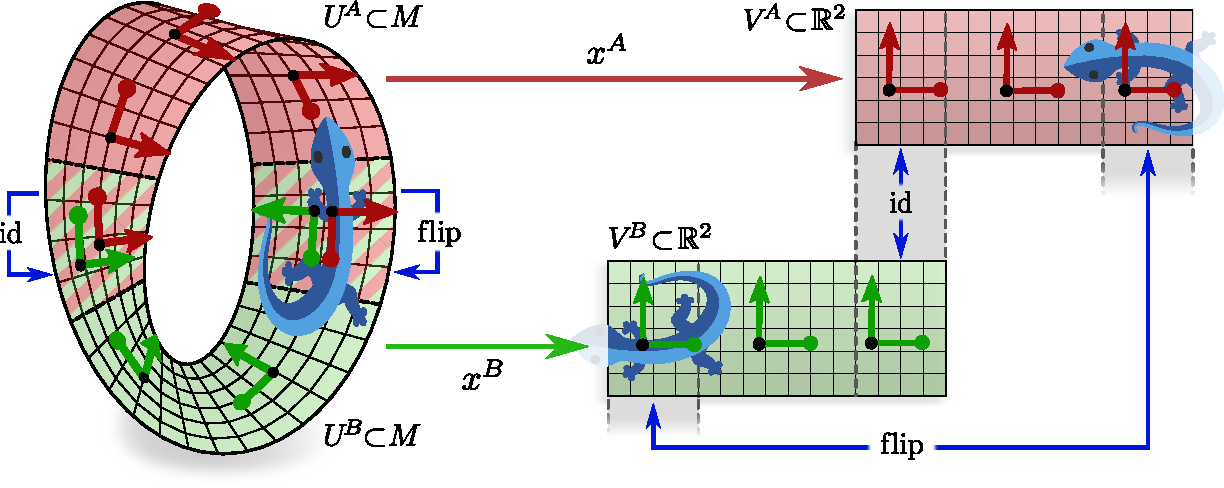
\includegraphics[width=\columnwidth]{figures/mobius_conv_gauges.pdf}
	\vspace*{.5ex}
	\caption{\small
		هندسه مسطح نوار موبیوس امکان زیرمجموعه‌های محلی را فراهم می‌کند که می‌توانند به‌طور ایزومتریک با زیرمجموعه‌های متناظر از~$\R^2$ شناسایی شوند.
		ما اطلسی ایزومتریک را ثابت می‌کنیم که از دو چارت $x^A$ و $x^B$ روی $U^A$ (قرمز) و $U^B$ (سبز) تشکیل می‌شود که کل نوار را می‌پوشانند.
		گیج‌های $\psi_p^X = \hat{d}x_p^X: \TpM \to \R^d$ برای $p\in U^A$ به‌عنوان دیفرانسیل‌های چارت القا می‌شوند.
		به دلیل پیچ نوار موبیوس، توابع گذار $g_p^{BA}$ در یکی از نواحی همپوشان بدیهی خواهند بود، در حالی که ناحیه دیگر لزوماً بین گیج‌ها از طریق انعکاس‌های~$s$ گذار خواهد کرد.
		اطلس انتخاب شده از چارت‌ها بنابراین $\Flip$-اطلسی از گیج‌ها را القا می‌کند و $\Flip$-ساختار متناظر $\RM$ را مستلزم می‌شود که از دو چارچوب منعکس‌شده در هر نقطه از~$M$ تشکیل می‌شود.
		هر یک از چارت‌های $x^X$ میدان چارچوب محلی هموار را القا می‌کند که توسط پایه‌های مختصاتی
		$\Big[\frac{\partial}{\partial x_i^X} \mkern-1mu\big|_p \Big] \raisebox{-2pt}{$\rule{0pt}{11pt}_{i=1}^d$}$
		داده می‌شود.
		انعکاس در توابع گذار در یک همپوشانی در انعکاس چارچوب‌ها نمایان می‌شود.
		{
			\\ \color{gray} \scriptsize
			(مارمولک‌ها تحت مجوز \lr{Creative Commons Attribution 4.0 International}
			\href{https://github.com/twitter/twemoji/blob/gh-pages/LICENSE-GRAPHICS}{\underline{\lr{license}}}
			با مجوز \lr{Twitter} اقتباس شده‌اند.)
		}
	}
	\label{fig:mobius_conv_gauges}
\end{figure}

اولین سؤالی که در ساخت \CNN مستقل از مختصات باید پاسخ داد این است که تا چه حد انتخاب چارچوب‌های مرجع مبهم است.
با توجه به متریک ریمانی روی نوار، می‌توانیم توجه خود را به چارچوب‌های متعامد محدود کنیم.
علاوه بر این می‌توان یکی از دو جهت \emph{در امتداد} نوار را متمایز کرد تا چرخش چارچوب‌های مرجع را با تراز کردن محورهای اول آنها با این جهت (به‌طور هموار) رفع ابهام کرد.
این ما را با ابهام دست‌گردی چارچوب باقی می‌گذارد، با دو جهت‌گیری که متناظر با دو جهت ممکن محور دوم چارچوب عمود بر نوار هستند.
نوار موبیوس به‌عنوان منیفلد غیرجهت‌پذیر، انتخاب سراسری هموار (یا حتی پیوسته) جهت‌گیری‌های چارچوب را نمی‌پذیرد.
برای به دست آوردن شهودی از این گزاره، تلاش برای ساخت میدان چارچوب هموار با انتخاب چارچوب دلخواه در موقعیت تصادفی و گسترش هموار این انتخاب روی کل نوار را در نظر بگیرید.
پس از یک دور کامل در اطراف نوار، چارچوب‌های ساخته‌شده ناگزیر نسبت به چارچوب‌های اولیه منعکس خواهند شد و بنابراین با هموار بودن مطلوب در تناقض خواهند بود.
بنابراین از نظر توپولوژیکی تعریف $\{e\}$-ساختار، یعنی میدان سراسری هموار چارچوب‌ها، روی نوار موبیوس \emph{غیرممکن} است.
بنابراین ما با گروه ساختار غیرقابل کاهش
\begin{align}
	G \,=\, \Flip \,\cong\, \Z/2\Z \,,
\end{align}
که انعکاس چارچوب‌ها را مدل می‌کند، باقی می‌مانیم.
گروه انعکاس فقط شامل دو عنصر است، همانی $e$ و انعکاس $s$، که طبق جدول ضرب ساده زیر ترکیب می‌شوند:
\begin{align}\label{eq:reflection_multiplication_table}
	\begin{tabular}{c|c@{\hspace{8pt}}c}
		& $e$ & $s$ \\ \hline
		$e$ & $e$ & $s$ \\
		$s$ & $s$ & $e$
	\end{tabular}
\end{align}
تنها گزاره غیربدیهی در این جدول این است که دو انعکاس یکدیگر را خنثی می‌کنند، یعنی $s^2=e$، یا به‌طور معادل، $s^{-1}=s$.
با توجه به غیرقابل کاهش بودن گروه ساختار $\Flip$، در ادامه باید $\Flip$-ساختار متناظر $\RM$ را در نظر بگیریم که از دو چارچوب با دست‌گردی مخالف در هر نقطه روی نوار موبیوس تشکیل می‌شود.

%!TEX root=../GaugeCNNTheory.tex

برای کدگذاری میدان‌های ویژگی مستقل از مختصات $\RM$ هموار روی $M$، نیاز است که $\Flip$-اطلسی مشخص شود که از گیج‌های مرتبط با $\Flip$ تشکیل شده و کل نوار را بپوشاند.
ما انتخاب می‌کنیم این کار را با ثابت کردن اطلسی از \emph{چارت‌ها}
\begin{align}
	x^X: U^X \to V^X \subset \R^2
\end{align}
که نوار را می‌پوشانند انجام دهیم و سپس گیج‌ها را از آن القا کنیم.
شکل~\ref{fig:mobius_conv_gauges} چنین اطلسی را تجسم می‌کند که از دو چارت $x^A$ و $x^B$ روی $U^A$ (قرمز) و $U^B$ (سبز) تشکیل شده است که دو نیمه همپوشان نوار را به‌طور ایزومتریک به نواحی مستطیلی متناظر از $\R^2$ نگاشت می‌کنند.
همانطور که در پیوست~\ref{apx:chart_induced_bases_main} توضیح داده شده، چارت‌ها گیج‌هایی را القا می‌کنند که توسط دیفرانسیل‌های چارت داده می‌شوند، یعنی
\begin{align}
	\psi_p^X \,:=\, \hat{d}x^X_p :\ \TpM \to \R^2 \ \ \ \textup{برای هر}\,\ p\in U^X\,\ \text{و}\,\ X=A,B \,.
\end{align}
توابع گذار سپس با ژاکوبین‌ها منطبق می‌شوند
$g^{BA} = \frac{\partial x^B}{\partial x^A}$.
به دلیل پیچ، نگاشت‌های گذار در یکی از دو ناحیه همپوشان همگی بدیهی هستند، یعنی $g_p^{BA} = e$، و در انتهای دیگر لزوماً منعکس هستند، یعنی $g_p^{BA} = s$.
اطلس القا شده از گیج‌ها بنابراین واقعاً به‌عنوان $\Flip$-اطلس شناسایی می‌شود.
از آنجا که از چارت‌های مختصاتی مشتق شده‌اند، میدان‌های چارچوب محلی هموار متناظر با گیج‌ها فقط پایه‌های مختصاتی معمول هستند، یعنی چارچوب‌های $\big[e_i^X \big]_{i=1}^d$ در $p\in U^X$ توسط
$\pig[\frac{\partial}{\partial x_i^X} \mkern-1mu\big|_p \pig] \raisebox{-2pt}{$\rule{0pt}{11pt}_{i=1}^d$}$
داده می‌شوند.
از آنجا که چارت‌ها ایزومتریک هستند، میدان چارچوب القا شده به‌طور خودکار متعامد است.
با این حال، دو ناحیه مستطیلی $V^A$ و $V^B$ در $\R^2$ نباید نسبت به یکدیگر چرخانده شوند تا $\Flip$-اطلس و $\Flip$-ساختار متناظر~$\RM$ را القا کنند.

باید تأکید کنیم که رویکرد القای گیج‌ها از طریق چارت‌های مختصاتی کاملاً ضروری نیست
-- این فقط گزینه‌ای مناسب است زیرا نوار موبیوس \emph{مسطح} به‌طور محلی با نواحی $\R^2$ به‌شکل \emph{ایزومتریک} شناسایی می‌شود.
این بعداً به ما اجازه خواهد داد تا شبکه‌های نمونه‌گیری منظم از $\R^2$، مانند شبکه پیکسل $\Z^2$، را به شبکه‌های نمونه‌گیری منظم روی نوار منتقل کنیم.
از آنجا که این برای منیفلدهایی که به‌طور محلی مسطح نیستند، مانند مِش‌ها در گرافیک کامپیوتری، ممکن نیست، اکثر پیاده‌سازی‌ها روی منیفلدهای عمومی (یا مِش‌ها) مختصات را مستقیماً به فضاهای مماس اختصاص می‌دهند؛ بخش~\ref{sec:instantiations_mesh} را ببینید.

اتصال کانونی لوی-چیویتا روی نوار موبیوس مفهوم انتقال موازی بردارهای مماس را تعریف می‌کند.
از آنجا که نوار به‌طور محلی با صفحه $\R^2$ ایزومتریک است، این انتقال می‌تواند روی تکه‌های محلی به‌عنوان مسطح کردن این تکه‌ها در یک صفحه و حرکت بردارها به‌طور معمول روی~$\R^2$ درک شود.
اگر هیچ تکه منفردی نتواند مسیر~$\gamma$ را بپوشاند، پوشش بازی وجود خواهد داشت که انتقال کامل توسط دنباله‌ای از انتقال‌دهنده‌ها روی تکه‌های محلی توضیح داده شود.
آسان است که دید انتقال نسبت به چارچوب‌های $\Flip$-ساختار انتخاب شده مقادیر $g_\gamma^{A\widetilde{A}}$ در گروه انعکاس $\Flip$ خواهد گرفت.
این بدان معنی است که اتصال لوی-چیویتا با~$\RM$ سازگار با $\Flip$ است.
بنابراین انتقال‌دهنده‌های خوش‌تعریف $\rho\big( g_\gamma^{A\widetilde{A}} \big)$ بردارهای ویژگی مرتبط با $\Flip$ را مستلزم می‌شود.

گروه $\IsomRM$ ایزومتری‌هایی که $\Flip$-ساختار را حفظ می‌کنند شامل تمام چرخش‌هایی است که نوار را در امتداد خودش جابه‌جا می‌کنند.
توجه کنید که یک چرخش یک‌بار در اطراف نوار، که آن را با زاویه $2\pi$ نشان می‌دهیم، با همانی مطابقت \emph{نمی‌کند} بلکه نوار را به‌شکل منعکس روی خودش نگاشت می‌کند.
تنها چرخش $4\pi$، یعنی دو دور کامل، نوار را به خودش بازمی‌گرداند.%
\footnote{
	بنابراین نوار موبیوس استوانه را به‌عنوان پوشش دوگانه در نظر می‌گیرد.
}
عمل گروه ایزومتری روی منیفلد و روی چارچوب‌های مرجع در شکل~\ref{fig:mobius_conv_isometries} تجسم شده است.
نسبت به مختصات، عمل ایزومتری تبدیل‌های گیج با مقادیر $\Flip$ را القا خواهد کرد.

\begin{figure}
	\centering
	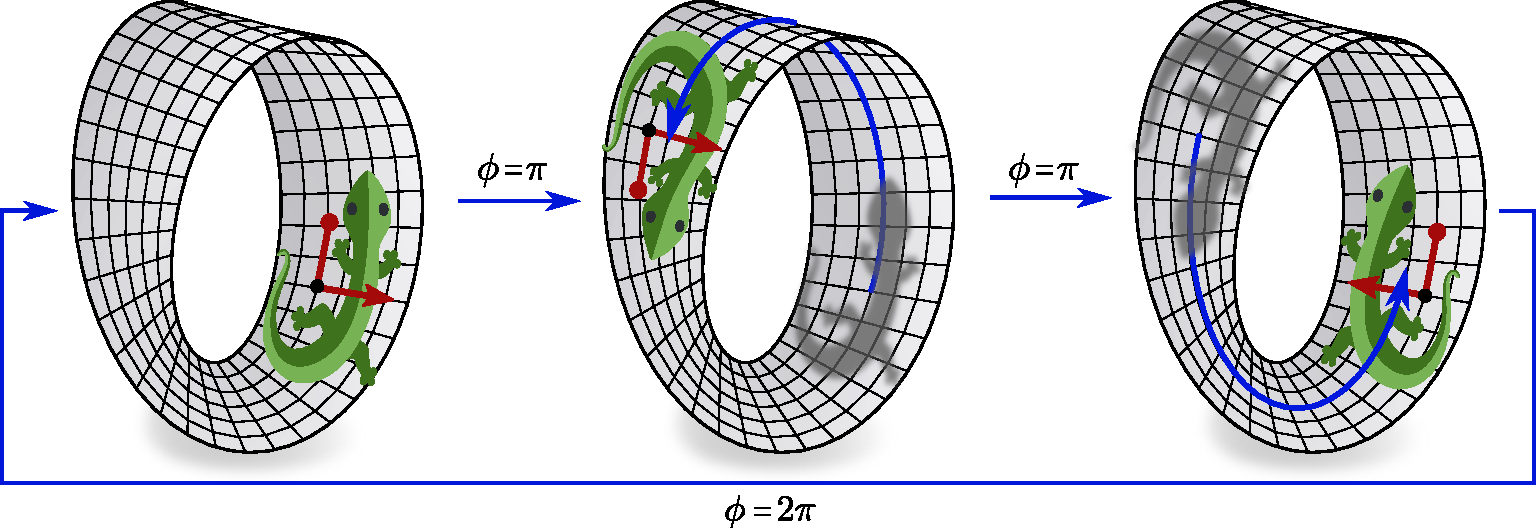
\includegraphics[width=\columnwidth]{figures/mobius_conv_isom.pdf}
	\caption{\small
		تجسم گروه ایزومتری‌های حافظ $\Flip$-ساختار $\IsomRM$ نوار موبیوس که با~$\SO2$ یکریخت است.
		این گروه شامل تمام چرخش‌ها در امتداد نوار است.
		به دلیل پیچ، چرخش $2\pi$، یعنی یک‌بار در اطراف نوار، هنوز آن را به خودش بازنمی‌گرداند بلکه منجر به انعکاس می‌شود.
		پس از دومین دور، یعنی چرخش کل $4\pi$، نوار به خودش بازمی‌گردد.
		تبدیل‌های گیج القا شده مقادیر در $\Flip$ می‌گیرند.
		{
			\\ \color{gray} \scriptsize
			(مارمولک‌ها تحت مجوز \lr{Creative Commons Attribution 4.0 International}
			\href{https://github.com/twitter/twemoji/blob/gh-pages/LICENSE-GRAPHICS}{\underline{\lr{license}}}
			با مجوز \lr{Twitter} اقتباس شده‌اند.)
		}
	}
	\label{fig:mobius_conv_isometries}
\end{figure}





%!TEX root=../GaugeCNNTheory.tex

\subsection{میدان‌های ویژگی مستقل از جهت‌گیری}
\label{sec:mobius_representations}

اصل کوواریانس مستلزم آن است که میدان‌های ویژگی روی نوار موبیوس مستقل از مختصات $\RM$ باشند، یعنی آنها باید به‌طور معادل نسبت به چارچوب‌های هر دو دست‌گردی قابل بیان باشند.
بنابراین آنها با انتخاب نمایش گروهی $\rho: \Flip \to \GL{c}$ از گروه انعکاس مشخص می‌شوند که تبدیل بردارهای ویژگی عددی هنگام تعویض بین دو جهت‌گیری را مشخص می‌کند.
در ادامه چند انتخاب ممکن از چنین انواع میدان‌هایی را مورد بحث قرار خواهیم داد.
خواننده ممکن است بخواهد بررسی کند که نمایش‌های پیشنهادی واقعاً همومورفیسم‌های گروهی هستند که $\rho(gh) = \rho(g)\rho(h)\,\ \forall\, g,h\in \Flip$ را برآورده می‌کنند، همانطور که در بخش~\ref{sec:feature_fields} و پاورقی~\ref{footnote:repr_group_homomorphism} خواسته شده است.

ابتدایی‌ترین مثال، که برای هر گروه ساختار وجود دارد، \emph{نمایش بدیهی} است
\begin{align}
	\rhotriv: \Flip \to \GL{1}\ , \qquad 
	\begin{aligned}
		e &\mapsto \big[\mkern2mu 1 \mkern2mu\big] \\[2pt]
		s &\mapsto \big[\mkern2mu 1 \mkern2mu\big] \\
	\end{aligned}
	\quad ,
\end{align}
که ماتریس همانی ${1\!\times\!1}$ را به هر دو عنصر گروه اختصاص می‌دهد.
این میدان‌های اسکالر $f_{\textup{triv}}$ را مدل می‌کند که از بردارهای ویژگی یک‌بعدی تشکیل شده‌اند که مختصات‌سازی‌های آنها $f^A_{\textup{triv}}(p) \in \R^1$ \emph{تحت انعکاس‌های چارچوب نامتغیر باقی می‌مانند}.
دومین نمایش یک‌بعدی، \emph{نمایش تغییر علامت} است
\begin{align}
	\rhosign: \Flip \to \GL{1}\ , \qquad 
	\begin{aligned}
		e &\mapsto \big[\mkern2mu 1 \mkern2mu\big] \\[2pt]
		s &\mapsto \big[\! \shortminus\!1 \big]
	\end{aligned}
	\quad .
\end{align}
این ماتریس همانی منفی ${1\!\times\!1}$ را به انعکاس‌ها اختصاص می‌دهد و بنابراین میدان‌های شبه‌اسکالر را توصیف می‌کند، یعنی میدان‌های ویژگی یک‌بعدی $f_{\textup{sign}}$ که ضرایب عددی آنها $f^A_{\textup{sign}}(p) \in \R^1$ \emph{تحت انعکاس‌ها علامت خود را تغییر می‌دهند}، \mbox{یعنی} ${\rhosign(s)\cdot f^A_{\textup{sign}}(p) = -f^A_{\textup{sign}}(p)}$.
از آنجا که نمایش بدیهی و نمایش تغییر علامت یک‌بعدی هستند، هر دو نمایش‌های غیرقابل کاهش (\lr{irreps}) گروه انعکاس هستند.
در واقع، آنها تنها دو \lr{irrep} گروه انعکاس هستند.%
\footnote{
	گروه انعکاس با گروه دوری $\Z/2\Z$ از مرتبه دو یکریخت است.
	به خوبی شناخته شده است که \lr{irrep}های گروه‌های دوری از مرتبه $N$ متناظر با ریشه‌های $N$ام وحدت هستند که برای $N=2$ فقط $+1$ (بدیهی) و $-1$ (تغییر علامت) هستند.
}

از آنجا که $\Flip$ گروه متناهی است، نمایش \emph{منظم} متناهی‌بعدی (دوبعدی) دارد
\begin{align}
	\rhoreg: \Flip \to \GL{2}\ , \qquad 
	\begin{aligned}
		e &\mapsto
		\begin{bmatrix} \hspace{1.5pt}
			1 &\mkern-4mu 0 \hspace*{1.5pt} \\ \hspace{1.5pt} 0 &\mkern-4mu 1 \hspace*{1.5pt}
		\end{bmatrix} \\[2pt]
		s &\mapsto 
		\begin{bmatrix} \hspace{1.5pt}
			0 &\mkern-4mu 1 \hspace*{1.5pt} \\ \hspace{1.5pt} 1 &\mkern-4mu 0 \hspace*{1.5pt}
		\end{bmatrix}
	\end{aligned}
	\quad ,
\end{align}
که عناصر گروه را توسط ماتریس‌های جایگشت نمایش می‌دهد.
طبق تعریف، نمایش منظم جایگشت عناصر گروه در $\Flip$ هنگام عمل بر خودشان را مدل می‌کند.
این را با ستون‌های جدول ضرب در معادله~\eqref{eq:reflection_multiplication_table} مقایسه کنید:
ستون میانی را می‌توان به‌عنوان ناشی از عمل $\rhoreg(e)$ بر ستون چپ در نظر گرفت، در حالی که عناصر گروه جابه‌جا شده در ستون راست متناظر با جایگشت توصیف شده توسط عمل $\rhoreg(s)$ بر ستون چپ هستند.
میدان‌های ویژگی منظم $f_{\textup{reg}}$ از $\Flip$ به‌طور عددی توسط بردارهای ویژگی دوبعدی $f^A_{\textup{reg}}(p) \in \R^2$ نمایش داده می‌شوند که دو \emph{کانال آنها تحت انعکاس‌ها جابه‌جا می‌شوند}، یعنی
$
\rhoreg(s) \mkern-1mu\cdot\mkern-2mu f^A_{\textup{reg}}(p)
\,=\,
\begin{bmatrix} \hspace{1.5pt} 0 &\mkern-4mu 1 \hspace*{1.5pt} \\ \hspace{1.5pt} 1 &\mkern-4mu 0 \hspace*{1.5pt} \end{bmatrix}
\mkern-4mu \cdot\mkern-4mu 
\begin{bmatrix} f^A_{\textup{reg},1} \\ f^A_{\textup{reg},2} \end{bmatrix} \!(p)
\,=\,
\begin{bmatrix} f^A_{\textup{reg},2} \\ f^A_{\textup{reg},1} \end{bmatrix} \!(p)
$.

نمایش منظم قابل کاهش است، یعنی شامل دو زیرفضای نامتغیر حقیقی است که در این مورد متناظر با نمایش بدیهی و نمایش تغییر علامت هستند.
بنابراین می‌توان آن را به‌طور معادل به‌عنوان ساخته شده از مجموع مستقیم $\rhotriv \oplus \rhosign$ آن دو \lr{irrep} و تغییر پایه $Q$ در نظر گرفت:
\begin{align}\label{eq:rho_reg_decomposition}
	\rhoreg(g)\ =\ Q\, \big( \rhotriv \!\oplus\mkern-1mu \rhosign \big)\mkern-2mu(g)\; Q^\top
	\quad\ \textup{که در آن } \quad
	Q = \frac{1}{\sqrt{2}}
	\begin{bmatrix} \hspace{1.5pt}
		1 &\mkern-7mu \shortminus1 \hspace*{1.5pt} \\ \hspace{1.5pt} 1 &\mkern-7mu \phantom{\shortminus}1 \hspace*{1.5pt}
	\end{bmatrix}
\end{align}
اعتبار این گزاره به‌آسانی با جایگذاری سمت راست برای هر دو عنصر گروه تأیید می‌شود:
\begin{align}
	Q\, \big( \rhotriv \!\oplus\mkern-1mu \rhosign \big)\mkern-2mu(e)\; Q^\top
	\ =\ \frac{1}{2}
	\begin{bmatrix} \hspace{1.5pt}
		1 &\mkern-7mu \shortminus1 \hspace*{1.5pt} \\ \hspace{1.5pt} 1 &\mkern-7mu \phantom{\shortminus}1 \hspace*{1.5pt}
	\end{bmatrix} \mkern-6mu \cdot\mkern-6mu
	\begin{bmatrix} \hspace{1.5pt}
		1 &\mkern-7mu 0 \hspace*{1.5pt} \\ \hspace{1.5pt} 0 &\mkern-7mu 1 \hspace*{1.5pt}
	\end{bmatrix} \mkern-6mu \cdot\mkern-6mu
	\begin{bmatrix} \hspace{1.5pt}
		\phantom{\shortminus}1 &\mkern-7mu 1 \hspace*{1.5pt} \\ \hspace{1.5pt} \shortminus1 &\mkern-7mu 1 \hspace*{1.5pt}
	\end{bmatrix}
	\ =\ 
	\begin{bmatrix} \hspace{1.5pt}
		1 &\mkern-7mu 0 \hspace*{1.5pt} \\ \hspace{1.5pt} 0 &\mkern-7mu 1 \hspace*{1.5pt}
	\end{bmatrix}
	\ =\ \rhoreg(e)
\end{align}
\begin{align}
	Q\, \big( \rhotriv \!\oplus\mkern-1mu \rhosign \big)\mkern-2mu(s)\; Q^\top
	\,=\, \frac{1}{2}
	\begin{bmatrix} \hspace{1.5pt}
		1 &\mkern-7mu \shortminus1 \hspace*{1.5pt} \\ \hspace{1.5pt} 1 &\mkern-7mu \phantom{\shortminus}1 \hspace*{1.5pt}
	\end{bmatrix} \mkern-6mu \cdot\mkern-6mu
	\begin{bmatrix} \hspace{1.5pt}
		1 &\mkern-7mu \phantom{\shortminus}0 \hspace*{1.5pt} \\ \hspace{1.5pt} 0 &\mkern-7mu \shortminus1 \hspace*{1.5pt}
	\end{bmatrix} \mkern-6mu \cdot\mkern-6mu
	\begin{bmatrix} \hspace{1.5pt}
		\phantom{\shortminus}1 &\mkern-7mu 1 \hspace*{1.5pt} \\ \hspace{1.5pt} \shortminus1 &\mkern-7mu 1 \hspace*{1.5pt}
	\end{bmatrix}
	\,=\, \frac{1}{2}
	\begin{bmatrix} \hspace{1.5pt}
		1 &\mkern-7mu \phantom{\shortminus}1 \hspace*{1.5pt} \\ \hspace{1.5pt} 1 &\mkern-7mu \shortminus1 \hspace*{1.5pt}
	\end{bmatrix} \mkern-6mu \cdot\mkern-6mu
	\begin{bmatrix} \hspace{1.5pt}
		\phantom{\shortminus}1 &\mkern-7mu 1 \hspace*{1.5pt} \\ \hspace{1.5pt} \shortminus1 &\mkern-7mu 1 \hspace*{1.5pt}
	\end{bmatrix}
	\,=\, 
	\begin{bmatrix} \hspace{1.5pt}
		0 &\mkern-7mu 1 \hspace*{1.5pt} \\ \hspace{1.5pt} 1 &\mkern-7mu 0 \hspace*{1.5pt}
	\end{bmatrix}
	\,=\, \rhoreg(s)
\end{align}
به‌طور کلی‌تر، هر نمایش متناهی‌بعدی گروه‌های فشرده (از جمله متناهی) \emph{کاملاً قابل کاهش} به مجموع مستقیم \lr{irrep}ها است~\cite{gallier2019harmonicRepr,din2017reprLectureNotes,serre1977linear}.
این نشان می‌دهد که هر بردار ویژگی کوواریانت که تحت گروه ساختار فشرده تبدیل می‌شود، تا حد تغییر پایه می‌تواند از ویژگی‌های \lr{irrep} ساخته شود.
همانطور که در~\cite{Weiler2019_E2CNN} استدلال شده است، در این مورد واقعاً امکان کاهش هر عملیات شبکه \emph{خطی} به عملیات معادل بین میدان‌های \lr{irrep} وجود دارد که ساخت فضای کرنل‌های $G$-راهبری‌پذیر در معادله~\eqref{eq:G-steerable_kernel_space} و بایاس‌های نامتغیر در معادله~\eqref{eq:gauge_bias_solution_space} را ساده می‌کند.
با این حال، همانطور که در ادامه خواهیم دید، انتخاب خاص پایه از انواع میدان معادل تأثیر کاملاً قابل توجهی بر عملکرد مدل دارد.
دلیل این امر آن است که عملیات شبکه \emph{غیرخطی} به پایه انتخاب شده حساس هستند، یعنی به انتخاب خاصی از انواع میدان معادل.

%!TEX root=../GaugeCNNTheory.tex

\subsection{شبکه‌های کانولوشنی مستقل از جهت‌گیری}
\label{sec:mobius_cnn_ops_analytical}

برای ساخت \lr{CNN}های مستقل از جهت‌گیری روی نوار موبیوس باید لایه‌های هم‌متغیر گیج از بخش~\ref{sec:gauge_CNNs_local} را برای گروه انعکاس~$\Flip$ نمونه‌سازی کنیم.
به‌طور مشخص‌تر، هر یک از توابع الگوی مشترک هم‌متغیر که لایه‌های مستقل از جهت‌گیری را تعریف می‌کنند باید برای هر انتخاب از انواع میدان در نظر گرفته شده $\rhotriv$، $\rhosign$ و $\rhoreg$ نمونه‌سازی شوند.
بخش~\ref{sec:mobius_bias} در ادامه با حل فضاهای $\mathscr{B}^R_\rho$ الگوهای بایاس نامتغیر گیج از معادله~\eqref{eq:gauge_bias_solution_space} شروع می‌کند.
چند انتخاب مجاز از غیرخطی‌های هم‌متغیر گیج برای انواع میدان مختلف در بخش~\ref{sec:mobius_nonlin} پیشنهاد می‌شوند.
بخش~\ref{sec:mobius_kernel_spaces} سپس فضاهای $\KR$ کرنل‌های $\Flip$-راهبری‌پذیر (معادله~\eqref{eq:G-steerable_kernel_space}) را برای هر جفت ممکن از \lr{irrep}های ورودی و خروجی استخراج خواهد کرد.
در حالی که این بخش عمدتاً شامل اشتقاقات نظری خواهد بود، بخش~\ref{sec:mobius_experiment_main} در ادامه جزئیات پیاده‌سازی عملی‌تری را پوشش خواهد داد.

\subsubsection{جمع بایاس مستقل از جهت‌گیری}
\label{sec:mobius_bias}

فضای الگوهای بایاس که می‌توانند به میدانی از نوع $\rho$ بدون دخالت در فرض استقلال از مختصات جمع شوند، در بخش~\ref{sec:gauge_bias_summation} نشان داده شد که توسط
\begin{align}
	\mathscr{B}^{\Flip}_\rho\ :=\ \big\{ b \in\R^c \;\big|\; b = \rho(g)\mkern2mu b\ \ \ \forall g\in \Flip \big\} \,.
\end{align}
داده می‌شود.
برای مورد گروه انعکاس، فقط دو عنصر گروه و بنابراین دو قید وجود دارد.
قید برای عنصر همانی $g=e$ به‌طور بدیهی برآورده می‌شود زیرا $\rho(e) = \id_{\R^c}$ طبق تعریف همیشه همانی روی~$\R^c$ است.
در ادامه بنابراین کافی است توجه را به قید $b = \rho(s)\mkern2mu b$ ناشی از انعکاس $g=s$ محدود کنیم.

با مورد میدان‌های اسکالر، یعنی نمایش بدیهی، شروع می‌کنیم.
قید انعکاس سپس $b = \rhotriv(s)\mkern2mu b = b$ می‌شود که همیشه برآورده می‌شود.
نتیجه می‌شود که فضای الگوهای بایاس
\begin{align}
	\mathscr{B}^{\Flip}_{\scalebox{.8}{$\rho_{{\textup{triv}}}$}} = \R
\end{align}
بدون قید باقی می‌ماند به‌طوری که بایاس‌های دلخواه با مقدار حقیقی می‌توانند به میدان‌های اسکالر جمع شوند.
برای نمایش تغییر علامت، قید انعکاس به $b = \rhotriv(s)\, b = -b$ تبدیل می‌شود و بنابراین فقط برای بایاس‌هایی که صفر هستند برآورده می‌شود:
\begin{align}
	\mathscr{B}^{\Flip}_{\scalebox{.8}{$\rho_{{\textup{sign}}}$}} = \{0\}
\end{align}
بنابراین جمع بایاس به میدان‌های تغییر علامت با حفظ استقلال از مختصات غیرممکن است.
سومین نوع میدان نمونه ما نمایش منظم دوبعدی است.
قید انعکاسی متناظر روی $b\in\R^2$ به صورت زیر است
\begin{align}
	\begin{bmatrix} b_1 \\ b_2 \end{bmatrix}
	\ =\ 
	b
	\ =\ 
	\rhoreg(s)\mkern2mu b
	\ =\ 
	\begin{bmatrix} \hspace{1.5pt}
		0 &\mkern-7mu 1 \hspace*{1.5pt} \\ \hspace{1.5pt} 1 &\mkern-7mu 0 \hspace*{1.5pt}
	\end{bmatrix}
	\!\cdot\! \begin{bmatrix} b_1 \\ b_2 \end{bmatrix}
	\ =\ 
	\begin{bmatrix} b_2 \\ b_1 \end{bmatrix}
\end{align}
و به فضای حل یک‌بعدی منجر می‌شود
\begin{align}\label{eq:bias_solution_space_regular}
	\mathscr{B}^{\Flip}_{\scalebox{.8}{$\rho_{{\textup{reg}}}$}} = 
	\big\{ b\in\R^2 \,\big|\, b_1=b_2 \big\} =
	\bigg\{ \begin{bmatrix} \beta \\ \beta \end{bmatrix} \,\bigg|\, \beta\in\R \bigg\} \ .
\end{align}
استقلال از مختصات این قید به‌طور شهودی روشن است:
از آنجا که نمایش منظم دو کانالی که میدان را تشکیل می‌دهند جابه‌جا می‌کند، جمع بایاس تنها زمانی مستقل از مختصات است که مقادیر جمع شده به هر دو کانال برابر باشند، به‌طوری که ترتیب آنها اهمیت نداشته باشد.

همانطور که قبلاً در بخش~\ref{sec:gauge_bias_summation} ادعا شد، فضای حل $\mathscr{B}^{\Flip}_\rho$ برای نمایش $\rho$ دقیقاً با زیرنمایش‌های بدیهی آن منطبق است.
این مطمئناً برای نمایش بدیهی صادق است که می‌توان هر بایاسی را به آن جمع کرد، و نمایش تغییر علامت که خود هیچ زیرنمایش بدیهی ندارد و بنابراین اصلاً بایاس نمی‌پذیرد.
مثال جالب‌تر نمایش منظم است که در معادله~\ref{eq:rho_reg_decomposition} نشان داده شد به مجموع مستقیم نمایش بدیهی و نمایش تغییر علامت تجزیه می‌شود.
فضای حل یک‌بعدی در معادله~\ref{eq:bias_solution_space_regular} دقیقاً متناظر با تک زیرنمایش بدیهی موجود در~$\rhoreg$ است.
برای بررسی اعتبار این گزاره، توجه کنید که بایاس‌های مجاز برای نمایش مجموع مستقیم $\rhotriv \oplus \rhosign$ از شکل $(\beta,\mkern1mu 0\mkern1mu)^\top$ هستند، که در آن $\beta\in\R$.
این نتیجه می‌تواند از طریق تغییر پایه $Q$ به نمایش منظم برگردانده شود که واقعاً حل ما در معادله~\eqref{eq:bias_solution_space_regular} را بازیابی می‌کند:
\begin{align}
	Q \cdot\mkern-2mu \begin{bmatrix} \beta \\ 0 \end{bmatrix}
	\ \propto\ 
	\begin{bmatrix} \hspace{1.5pt}
		1 &\mkern-7mu \shortminus1 \hspace*{1.5pt} \\ \hspace{1.5pt} 1 &\mkern-7mu \phantom{\shortminus}1 \hspace*{1.5pt}
	\end{bmatrix}
	\!\cdot\! \begin{bmatrix} \beta \\ 0 \end{bmatrix}
	\ =\ 
	\begin{bmatrix} \beta \\ \beta \end{bmatrix}
\end{align}





%!TEX root=../GaugeCNNTheory.tex

\subsubsection{غیرخطی‌های مستقل از جهت‌گیری}
\label{sec:mobius_nonlin}

برای ساخت شبکه عمیق، باید غیرخطی‌های هم‌متغیر برای هر یک از انواع میدان ارائه دهیم.
همانطور که قبلاً در بخش~\ref{sec:gauge_nonlinearities} بحث شد، میدان‌های اسکالر به دلیل نامتغیر بودن آنها تحت تبدیل‌های گیج می‌توانند تحت تأثیر هر غیرخطی $\mathscr{s}_{\textup{triv}}: \R\to\R$ قرار بگیرند.
انتخاب‌های معمول غیرخطی‌های نقطه‌ای \lr{ReLU} یا \lr{ELU} هستند.
برای میدان‌های تغییر علامت می‌توان قدر مطلق $\lVert f^A_{\textup{sign}}(p) \rVert$ بردارهای ویژگی را که میدان تغییر علامت را به میدان اسکالر نگاشت می‌کند، در نظر گرفت.
در پیاده‌سازی ما در ادامه به جای آن از غیرخطی‌هایی از شکل
\begin{align}\label{eq:signflip_nonlin}
	\mathscr{s}_{\textup{sign}}: \mathscr{f} \ \mapsto\ 
	\operatorname{ReLU} \!\big( \lVert \mathscr{f} \rVert - b \big) \mkern-2mu\cdot\!
	\frac{\mathscr{f}}{\lVert \mathscr{f} \rVert},
\end{align}
استفاده می‌کنیم، که در آن $b\in\R^+$ پارامتر بایاس قابل آموزش است.
به‌آسانی دیده می‌شود که این انتخاب میدان‌های تغییر علامت را به میدان‌های تغییر علامت نگاشت می‌کند زیرا ضریب اول بر روی نرم نامتغیر گیج بردارهای ویژگی عمل می‌کند در حالی که ضریب دوم علامت بردار ویژگی را حفظ می‌کند.
به‌عنوان نمایش جایگشت، نمایش منظم اجازه می‌دهد هر غیرخطی نقطه‌ای، مثلاً \lr{ReLU}ها، بر روی کانال‌های میدان منفرد بدون تغییر نوع میدان عمل کند:
\begin{align}
	\rhoreg(s) \circ \mathscr{s}_{\textup{reg}} \begin{bmatrix} \mathscr{f}_1 \\ \mathscr{f}_2 \end{bmatrix}
	\ =\ 
	\begin{bmatrix} \hspace{1.5pt}
		0 &\mkern-7mu 1 \hspace*{1.5pt} \\ \hspace{1.5pt} 1 &\mkern-7mu 0 \hspace*{1.5pt}
	\end{bmatrix}
	\begin{bmatrix} \operatorname{ReLU}(\mathscr{f}_1) \\ \operatorname{ReLU}(\mathscr{f}_2) \end{bmatrix}
	\ =\ 
	\begin{bmatrix} \operatorname{ReLU}(\mathscr{f}_2) \\ \operatorname{ReLU}(\mathscr{f}_1) \end{bmatrix}
	\ =\ 
	\mathscr{s}_{\textup{reg}} \begin{bmatrix} \mathscr{f}_2 \\ \mathscr{f}_1 \end{bmatrix}
	\ =\ 
	\mathscr{s}_{\textup{reg}} \circ \rhoreg(s) \begin{bmatrix} \mathscr{f}_1 \\ \mathscr{f}_2 \end{bmatrix}
\end{align}
در حالی که نمایش منظم از نظر خطی معادل $\rhotriv\oplus\rhosign$ است، نمی‌توانیم غیرخطی‌های نقطه‌ای مستقل را روی دو کانال در پایه \lr{irrep} اعمال کنیم.
این ادعا را که غیرخطی‌ها شبکه‌ها را نسبت به انتخاب خاص پایه نمایش حساس می‌کنند، تقویت می‌کند.

\subsubsection{کانولوشن‌های مستقل از جهت‌گیری}
\label{sec:mobius_kernel_spaces}

آخرین عملیاتی که اینجا نمونه‌سازی می‌کنیم کانولوشن‌های هم‌متغیر انعکاس هستند.
این از یک طرف مستلزم توضیح نگاشت نمایی و انتقال موازی روی نوار است، و از طرف دیگر حل فضاهای کرنل $\Flip$-راهبری‌پذیر.
به دلیل هندسه مسطح $M$ و استفاده از چارت‌های ایزومتریک، مورد اول تقریباً بدیهی است:
ویژگی‌ها مشابه روی $\R^2$ منتقل می‌شوند، با این تفاوت که بردارهای ویژگی ممکن است انعکاسی توسط~$\rho(s)$ تجربه کنند.
پیاده‌سازی ما از این بخش در شکل~\ref{fig:mobius_conv_numerical} تجسم شده است که در بخش~\ref{sec:mobius_implementation} در ادامه بیشتر توضیح داده می‌شود.
بخش فعلی انحصاراً بر حل تحلیلی فضاهای کرنل متمرکز است.

برای نوار موبیوس با $\Flip$-ساختار، فضای کرنل‌های $\Flip$-راهبری‌پذیر از معادله~\eqref{eq:G-steerable_kernel_space} توسط
\begin{align}
	\KR :=\ \Big\{ K\!: \R^2 \to \R^{\cout\times\cin} \,\Big|\,
	K(g\mkern1mu\mathscr{v}) = \rhoout(g) \mkern-2mu\cdot\mkern-2mu K(\mathscr{v}) \mkern-2mu\cdot\mkern-2mu \rhoin(g) \quad \forall\ \mathscr{v} \in \R^2,\,\ g\in \Flip \Big\} \,,
\end{align}
داده می‌شود، که در آن ضریب دترمینان $\detg=1$ را حذف کردیم و تمام معکوس‌ها را برداشتیم زیرا ${g^{-1} \!=\! g\ \ \ \forall\mkern4mu g \in \Flip}$.
همانند مورد بایاس‌های هم‌متغیر، قید ناشی از عنصر همانی به‌طور بدیهی برآورده می‌شود، به‌طوری که فقط قید انعکاسی باقی می‌ماند.
کرنل‌های هم‌متغیر انعکاس بنابراین با قید واحد
\begin{align}
	K(s.\mathscr{v})\ =\ \rhoout(s) \mkern-1mu\cdot\mkern-1mu K(\mathscr{v}) \mkern-1mu\cdot\mkern-1mu \rhoin(s) \qquad \forall\: \mathscr{v} \in \R^2 \,,
\end{align}
مشخص می‌شوند، که مستلزم آن است که کرنل منعکس‌شده $K(s.\mathscr{v})$ برابر کرنل منعکس نشده $K(\mathscr{v})$ پس از عمل نمایش میدان ورودی و خروجی باشد.
در ادامه این قید را برای تمام نه جفت از انواع میدان حل خواهیم کرد.
کرنل‌های حاصل، که همگی به نحوی متقارن تحت انعکاس‌ها هستند، در جدول~\ref{tab:reflection_steerable_kernels} تجسم شده‌اند.

\begin{SCtable}
	\hspace*{-5.ex}
	\def\figfolder{figures/kernels/}
	\def\figheight{0.08\columnwidth}
	\newlength{\vertSkip}
	\newlength{\eqToKernelSkip}
	\setlength\vertSkip{4.5ex}
	\setlength\eqToKernelSkip{1.5ex}
	\newcommand\cellTstrut{\rule{0pt}{3.5ex}}
	\footnotesize
	\setlength{\tabcolsep}{4pt}
	\begin{tabular}{r|c|c|c}
		\diagbox[height=18pt]{\raisebox{3pt}{$\rhoout$}}{\raisebox{-0pt}{$\rhoin$}}
		& بدیهی & تغییر علامت & منظم \\
		\hline
		\cellTstrut
		%%%%%%%%%%%%%% FIRST ROW %%%%%%%%%%%%%%%
		\multirow{2}{*}{
			\hspace*{-1.5ex}
			بدیهی
			\hspace*{-1ex}
			\rule{0pt}{5.5ex}
		}
		& $\Koo(s.\mathscr{v}) = \Koo(\mathscr{v})$
		& $\Koo(s.\mathscr{v}) = \minus\Koo(\mathscr{v})$
		& $\Koo(s.\mathscr{v}) = \Kot(\mathscr{v})$
		\\[\eqToKernelSkip]
		& $\begin{pmatrix} \includegraphicstotab[height=\figheight]{\figfolder K_symmetric.png} \end{pmatrix}$
		& $\begin{pmatrix} \includegraphicstotab[height=\figheight]{\figfolder K_antisymmetric.png} \end{pmatrix}$
		& $\begin{pmatrix}
			\includegraphicstotab[height=\figheight]{\figfolder K_crisp_1.png} \mkern4mu, & \mkern-16mu
			\includegraphicstotab[height=\figheight]{\figfolder K_crisp_1f.png}
		\end{pmatrix}$ 
		\hspace{-6pt}
		\\[\vertSkip]
		\hline
		\cellTstrut
		%%%%%%%%%%%%%% SECOND ROW %%%%%%%%%%%%%%%
		\multirow{2}{*}{
			\hspace*{-1.5ex}
			تغییر علامت
			\hspace*{-1ex}
			\rule{0pt}{5.5ex}
		}
		& $\Koo(s.\mathscr{v}) = \minus\Koo(\mathscr{v})$
		& $\Koo(s.\mathscr{v}) = \Koo(\mathscr{v})$
		& $\Koo(s.\mathscr{v}) = \minus\Kot(\mathscr{v})$
		\\[\eqToKernelSkip]
		& $\begin{pmatrix} \includegraphicstotab[height=\figheight]{\figfolder K_antisymmetric.png} \end{pmatrix} $
		& $\begin{pmatrix} \includegraphicstotab[height=\figheight]{\figfolder K_symmetric.png} \end{pmatrix} $
		& $\begin{pmatrix}
			\includegraphicstotab[height=\figheight]{\figfolder K_crisp_1.png} \mkern4mu, & \mkern-16mu
			\includegraphicstotab[height=\figheight]{\figfolder K_crisp_1f_inverted.png}
		\end{pmatrix} $ 
		\hspace{-6pt}
		\\[\vertSkip]
		\hline
		\rule{0pt}{5.ex}
		%%%%%%%%%%%%%% THIRD ROW %%%%%%%%%%%%%%%
		\multirow{2}{*}{
			\hspace*{-1.5ex}
			منظم
			\hspace*{-1ex}
			\rule{0pt}{10.5ex}
		}
		& $\Koo(s.\mathscr{v}) = \Kto(\mathscr{v})$
		& $\Koo(s.\mathscr{v}) = \minus\Kto(\mathscr{v})$
		& \makecell{
			$\Koo(s.\mathscr{v}) = \Ktt(\mathscr{v})$ \\[.6ex]
			$\Kot(s.\mathscr{v}) = \Kto(\mathscr{v})$
		}
		\hspace{-6pt}
		\\[3.ex]
		& $\begin{pmatrix}
			\includegraphicstotab[height=\figheight]{\figfolder K_crisp_1.png} \\
			\includegraphicstotab[height=\figheight]{\figfolder K_crisp_1f.png}
		\end{pmatrix}$
		& $\begin{pmatrix}
			\includegraphicstotab[height=\figheight]{\figfolder K_crisp_1.png} \\
			\includegraphicstotab[height=\figheight]{\figfolder K_crisp_1f_inverted.png}
		\end{pmatrix}$
		& $\begin{pmatrix}
			\includegraphicstotab[height=\figheight]{\figfolder K_crisp_1.png} \mkern4mu, & \mkern-16mu
			\includegraphicstotab[height=\figheight]{\figfolder K_crisp_3.png} \\
			\includegraphicstotab[height=\figheight]{\figfolder K_crisp_3f.png} \mkern4mu, & \mkern-16mu
			\includegraphicstotab[height=\figheight]{\figfolder K_crisp_1f.png}
		\end{pmatrix}$
	\end{tabular}
	%%%%%%%%%%%%%%%%%%%%%%%%%%%%%%%%%%%%%%%%%%%%%%%%%%%%%%%%%%%%%%%%%%%%%%%%%%%%%%%%%%%%%%%%%%%%%%%%%%%%%%%
	\captionsetup{width=1.\textwidth}
	\caption[]{\small
		\protect\rule{0ex}{8ex} % vertical position
		تجسم کرنل‌های انعکاس-راهبری‌پذیر در $\KR$ برای تمام جفت‌های در نظر گرفته شده از انواع میدان ورودی و خروجی $\rhoin$ و $\rhoout$.
		به‌طور کلی، این کرنل‌ها باید قید کرنل $\Flip\mkern-1.2mu$-راهبری‌پذیری $K(s.\mathscr{v})\ =\ \rhoout(s) \mkern-1mu\cdot\mkern-1mu K(\mathscr{v}) \mkern-1mu\cdot\mkern-1mu \rhoin(s)$ را برآورده کنند که در آن $K: \R^2 \to \R^{\cout\times\cin}$.
		هر ورودی جدول قید خاص برای نمایش‌های ورودی و خروجی متناظر را بیان می‌کند و یک کرنل راهبری‌پذیر نمونه را تجسم می‌کند.
		توجه کنید که قید، کرنل منعکس‌شده $K(s.\mathscr{v})$ را به تبدیل خطی کرنل منعکس نشده $K(\mathscr{v})$ توسط نمایش ورودی و خروجی مقید می‌کند.
		بنابراین منجر به تقارن‌های انعکاسی کرنل‌ها می‌شود.
	}
	\label{tab:reflection_steerable_kernels}
\end{SCtable}


\begin{itemize}
	\setlength{\itemindent}{-2em}
	\setlength{\itemsep}{.5em}
	\item[{\rule[2.0pt]{2pt}{2pt}}]
	\textbf{اسکالر $\leftarrow$ اسکالر:}
	کرنل‌های
	$K = \pig[\Koo\pig]: \R^2 \to \R^{1\times1}$
	که بین میدان‌های اسکالر نگاشت می‌کنند باید محدودیت زیر را برآورده کنند
	\begin{align}
		\pig[\Koo\pig] \mkern-1mu (s.\mathscr{v})
		\ =\ 
		\big[\mkern2mu 1 \mkern2mu\big]
		\!\cdot\!
		\pig[\Koo\pig] \mkern-1mu (\mathscr{v})
		\cdot\!
		\big[\mkern2mu 1 \mkern2mu\big]
		\ =\ 
		\pig[\Koo\pig] \mkern-1mu (\mathscr{v})
		\qquad \forall\ \mathscr{v} \in \R^2 \,.
	\end{align}
	آنها لزوماً تحت بازتاب‌ها \emph{متقارن} (ناوردا) هستند؛ ورودی سمت چپ بالا در جدول~\ref{tab:reflection_steerable_kernels} را ببینید.
	\item[{\rule[2.0pt]{2pt}{2pt}}]
	\textbf{اسکالر $\leftarrow$ علامت-چرخش:}
	کرنل‌های $K = \pig[\Koo\pig]: \R^2 \to \R^{1\times1}$ که میدان اسکالر را به میدان علامت-چرخش نگاشت می‌کنند باید محدودیت زیر را برآورده کنند
	\begin{align}
		\pig[\Koo\pig] \mkern-1mu (s.\mathscr{v})
		\ =\ 
		\big[\! \shortminus\!1 \big]
		\!\cdot\!
		\pig[\Koo\pig] \mkern-1mu (\mathscr{v})
		\cdot\!
		\big[\mkern2mu 1 \mkern2mu\big]
		\ =\
		-\pig[\Koo\pig] \mkern-1mu (\mathscr{v})
		\qquad \forall\ \mathscr{v} \in \R^2 \,.
	\end{align}
	این امر کرنل‌های \emph{ضدمتقارن} را به همراه دارد همانطور که در ردیف وسط در ستون اول جدول~\ref{tab:reflection_steerable_kernels} مشاهده می‌شود.
	\item[{\rule[2.0pt]{2pt}{2pt}}]
	\textbf{اسکالر $\leftarrow$ منظم:}
	به منظور نگاشت از میدان اسکالر به میدان ویژگی منظم، باید کرنل‌هایی از شکل
	$K = \begin{bmatrix} \Koo \\ \Kto \end{bmatrix}: \R^2 \to \R^{2\times1}$
	که از یک کانال ورودی به دو کانال خروجی نگاشت می‌کند، اعمال کرد.
	جایگشت مورد نیاز کانال‌های خروجی در صورتی تضمین می‌شود که کرنل محدودیت زیر را برآورده کند
	\begin{align}\label{eq:constraint_s2r}
		\begin{bmatrix} \Koo \\ \Kto \end{bmatrix} \mkern-4mu (s.\mathscr{v})
		\ =\ 
		\begin{bmatrix} \hspace{1.5pt} 0 &\mkern-4mu 1 \hspace*{1.5pt} \\ \hspace{1.5pt} 1 &\mkern-4mu 0 \hspace*{1.5pt} \end{bmatrix}
		\!\cdot\!
		\begin{bmatrix} \Koo \\ \Kto \end{bmatrix} \mkern-4mu (\mathscr{v})
		\cdot\!
		\big[\mkern2mu 1 \mkern2mu\big]
		\ =\ 
		\begin{bmatrix} \Kto \\ \Koo \end{bmatrix} \mkern-4mu (\mathscr{v})
		\qquad \forall\ \mathscr{v} \in \R^2 \,.
	\end{align}
	این محدودیت مستلزم آن است که دو کانال حاوی کرنل‌هایی باشند که \emph{نسخه‌های بازتابی} یکدیگر هستند، یعنی
	$\Koo(s.\mathscr{v}) = \Kto(\mathscr{v})$ برای همه $\mathscr{v} \in \R^2$
	(این قبلاً خط دوم محدودیت در معادله~\eqref{eq:constraint_s2r} را پوشش می‌دهد).
	این حالت در ورودی سمت چپ پایین جدول~\ref{tab:reflection_steerable_kernels} مشاهده می‌شود.
	%%%%%%%%%%%%%%%%%%%%%%%%%%%%%%%%%%%%%%%%%%%%%%%%%%%%%%%%%%%%%%%%%%%%%%%%%%%%%%%%%%%%%%%%%%%%%%%%%%%%%%
	\item[{\rule[2.0pt]{2pt}{2pt}}]
	\textbf{علامت-چرخش $\leftarrow$ اسکالر:}
	کرنل‌های
	$K = \pig[\Koo\pig]: \R^2 \to \R^{1\times1}$
	که از علامت-چرخش به میدان‌های اسکالر نگاشت می‌کنند دوباره \emph{ضدمتقارن} هستند زیرا باید همان محدودیت را برآورده کنند
	\begin{align}
		\pig[\Koo\pig] \mkern-1mu (s.\mathscr{v})
		\ =\ 
		\big[\mkern2mu 1 \mkern2mu\big]
		\!\cdot\!
		\pig[\Koo\pig] \mkern-1mu (\mathscr{v})
		\cdot\!
		\big[\! \shortminus\!1 \big]
		\ =\ 
		-\pig[\Koo\pig] \mkern-1mu (\mathscr{v})
		\qquad \forall\ \mathscr{v} \in \R^2
	\end{align}
	مانند کرنل‌هایی که در جهت مخالف نگاشت می‌کنند.
	\item[{\rule[2.0pt]{2pt}{2pt}}]
	\textbf{علامت-چرخش $\leftarrow$ علامت-چرخش:}
	کرنل‌های
	$K = \pig[\Koo\pig]: \R^2 \to \R^{1\times1}$
	که رفتار تبدیل میدان‌های علامت-چرخش را حفظ می‌کنند \emph{متقارن} هستند زیرا دو وارونگی علامت در محدودیت
	\begin{align}
		\pig[\Koo\pig] \mkern-1mu (s.\mathscr{v})
		\ =\ 
		\big[\! \shortminus\!1 \big]
		\!\cdot\!
		\pig[\Koo\pig] \mkern-1mu (\mathscr{v})
		\cdot\!
		\big[\! \shortminus\!1 \big]
		\ =\ 
		\pig[\Koo\pig] \mkern-1mu (\mathscr{v})
		\qquad \forall\ \mathscr{v} \in \R^2
	\end{align}
	حذف می‌شوند.
	\item[{\rule[2.0pt]{2pt}{2pt}}]
	\textbf{علامت-چرخش $\leftarrow$ منظم:}
	در حالت کرنل‌های
	$K = \begin{bmatrix} \Koo \\ \Kto \end{bmatrix}: \R^2 \to \R^{2\times1}$
	که از علامت-چرخش به میدان‌های ویژگی منظم نگاشت می‌کند، محدودیت زیر بدست می‌آید
	\begin{align}
		\begin{bmatrix} \Koo \\ \Kto \end{bmatrix} \mkern-4mu (s.\mathscr{v})
		\ =\ 
		\begin{bmatrix} \hspace{1.5pt} 0 &\mkern-4mu 1 \hspace*{1.5pt} \\ \hspace{1.5pt} 1 &\mkern-4mu 0 \hspace*{1.5pt} \end{bmatrix}
		\!\cdot\!
		\begin{bmatrix} \Koo \\ \Kto \end{bmatrix} \mkern-4mu (\mathscr{v})
		\cdot\!
		\big[\! \shortminus\!1 \big]
		\ =\ 
		- \begin{bmatrix} \Kto \\ \Koo \end{bmatrix} \mkern-4mu (\mathscr{v})
		\qquad \forall\ \mathscr{v} \in \R^2 \,.
	\end{align}
	دو خط با یکدیگر مطابقت دارند، به طوری که می‌توان آنها را با محدودیت کرنل یگانه
	${\Koo(s.\mathscr{v}) = -\Kto(\mathscr{v})}\ \ \forall \mathscr{v}\in \R^2$ خلاصه کرد.
	این محدودیت مستلزم آن است که دو کانال کرنل حاوی \emph{نسخه‌های بازتابی، منفی شده} یکدیگر باشند؛ تجسم آن در وسط ردیف پایین جدول~\ref{tab:reflection_steerable_kernels} را ببینید.
	%%%%%%%%%%%%%%%%%%%%%%%%%%%%%%%%%%%%%%%%%%%%%%%%%%%%%%%%%%%%%%%%%%%%%%%%%%%%%%%%%%%%%%%%%%%%%%%%%%%%%%
	\item[{\rule[2.0pt]{2pt}{2pt}}]
	\textbf{منظم $\leftarrow$ اسکالر:}
	کرنل‌هایی که میدان‌های ویژگی منظم را به میدان‌های اسکالر نگاشت می‌کنند دارای دو کانال ورودی و یک کانال خروجی هستند و بنابراین از شکل
	$K = \pig[\Koo \,,\, \Kot\pig]: \R^2 \to \R^{1\times2}$ هستند.
	محدودیت
	\begin{align}
		\pig[\Koo \,,\, \Kot\pig] \mkern-1mu (s.\mathscr{v})
		\ =\ 
		\big[\mkern2mu 1 \mkern2mu\big]
		\!\cdot\!
		\pig[\Koo \,,\, \Kot\pig] \mkern-1mu (\mathscr{v})
		\cdot\!
		\begin{bmatrix} \hspace{1.5pt} 0 &\mkern-4mu 1 \hspace*{1.5pt} \\ \hspace{1.5pt} 1 &\mkern-4mu 0 \hspace*{1.5pt} \end{bmatrix}
		\ =\ 
		\pig[\Kot \,,\, \Koo\pig] \mkern-1mu (\mathscr{v})
		\qquad \forall\ \mathscr{v} \in \R^2 \,,
	\end{align}
	که می‌توان آن را به الزام
	$\Koo(s.\mathscr{v}) = \Kot(\mathscr{v})\ \ \forall \mathscr{v} \in \R^2$ کاهش داد،
	دوباره مستلزم آن است که دو ورودی کرنل حاوی \emph{نسخه‌های بازتابی} یکدیگر باشند.
	\item[{\rule[2.0pt]{2pt}{2pt}}]
	\textbf{منظم $\leftarrow$ علامت-چرخش:}
	نگاشت‌هایی از میدان‌های ویژگی منظم به میدان‌های علامت-چرخش از کرنل‌های
	$K = \pig[\Koo,\, \Kot\pig]: \R^2 \to \R^{1\times2}$
	که محدودیت زیر را برآورده می‌کنند استفاده می‌کنند
	\begin{align}
		\pig[\Koo \,,\, \Kot\pig] \mkern-1mu (s.\mathscr{v})
		\ =\ 
		\big[\! \shortminus\!1 \big]
		\!\cdot\!
		\pig[\Koo \,,\, \Kot\pig] \mkern-1mu (\mathscr{v})
		\cdot\!
		\begin{bmatrix} \hspace{1.5pt} 0 &\mkern-4mu 1 \hspace*{1.5pt} \\ \hspace{1.5pt} 1 &\mkern-4mu 0 \hspace*{1.5pt} \end{bmatrix}
		\ =\ 
		- \pig[\Kot \,,\, \Koo\pig] \mkern-1mu (\mathscr{v})
		\qquad \forall\ \mathscr{v} \in \R^2 \,,
	\end{align}
	یا معادل آن، $\Koo(s.\mathscr{v}) = -\Kot(\mathscr{v})\ \ \forall \mathscr{v} \in \R^2$.
	احتمالاً همانطور که قبلاً انتظار می‌رفت، آنها از کرنل‌هایی تشکیل شده‌اند که دو کانال آنها حاوی \emph{نسخه‌های بازتابی، منفی شده} یکدیگر هستند.
	\item[{\rule[2.0pt]{2pt}{2pt}}]
	\textbf{منظم $\leftarrow$ منظم:}
	در نهایت، باید کرنل‌های
	$K = \begin{bmatrix} \Koo &\mkern-12mu \Kot \\ \Kto &\mkern-12mu \Ktt \end{bmatrix}: \R^2 \to \R^{2\times2}$
	که میدان‌های منظم را به میدان‌های منظم نگاشت می‌کنند و بنابراین دارای ماتریس‌های $2\times2$ به عنوان کودومین هستند، در نظر بگیریم.
	محدودیت آنها، که از ضرب چپ و راست با نمایش منظم حاصل می‌شود، به شکل زیر است
	\begin{align}
		\begin{bmatrix} \Koo &\mkern-12mu \Kot \\ \Kto &\mkern-12mu \Ktt \end{bmatrix} \mkern-4mu (s.\mathscr{v})
		\ =\ 
		\begin{bmatrix} \hspace{1.5pt} 0 &\mkern-4mu 1 \hspace*{1.5pt} \\ \hspace{1.5pt} 1 &\mkern-4mu 0 \hspace*{1.5pt} \end{bmatrix}
		\!\cdot\!
		\begin{bmatrix} \Koo &\mkern-12mu \Kot \\ \Kto &\mkern-12mu \Ktt \end{bmatrix} \mkern-4mu (\mathscr{v})
		\cdot\!
		\begin{bmatrix} \hspace{1.5pt} 0 &\mkern-4mu 1 \hspace*{1.5pt} \\ \hspace{1.5pt} 1 &\mkern-4mu 0 \hspace*{1.5pt} \end{bmatrix}
		\ =\ 
		\begin{bmatrix} \Ktt &\mkern-12mu \Kto \\ \Kot &\mkern-12mu \Koo \end{bmatrix} \mkern-4mu (\mathscr{v})
		\qquad \forall\ \mathscr{v} \in \R^2 \,.
	\end{align}
	این معادل دو محدودیت مستقل است
	\begin{align}
		\Koo(s.\mathscr{v}) = \Ktt(\mathscr{v}) \quad \forall \mathscr{v} \in \R^2
	\end{align}
	و
	\begin{align}
		\Kot(s.\mathscr{v}) = \Kto(\mathscr{v}) \quad \forall \mathscr{v} \in \R^2 \,,
	\end{align}
	که چهار ورودی کرنل را به هم متصل می‌کند به طوری که \emph{دو جفت کرنل منعکس شده متقابل} وجود دارد.
	این حالت در ورودی سمت راست پایین جدول~\ref{tab:reflection_steerable_kernels} مشاهده می‌شود.
\end{itemize}

در حالی که نتایج استخراج شده به ما می‌گویند چگونه بین میدان‌های ویژگی منفرد نگاشت کنیم، شبکه‌های عصبی معمولاً فضاهای ویژگی را فرض می‌کنند که از چندین میدان ویژگی احتمالاً متفاوت تشکیل می‌شوند.
کرنل‌هایی که بین این پشته‌های میدان‌های ویژگی نگاشت می‌کنند را می‌توان به‌عنوان ساخته شده از بلوک‌هایی در نظر گرفت که بین میدان‌های منفرد نگاشت می‌کنند.
به‌عنوان مثال، موردی را در نظر بگیرید که هر دو فضای ویژگی ورودی و خروجی شامل یکی از نمایش‌های مورد بحث هستند، یعنی $\rhoin = \rhoout = \rhotriv \oplus \rhosign \oplus \rhoreg$.
تعداد کانال‌های ورودی و خروجی سپس $\cin=\cout=1+1+2=4$ است، به‌طوری که کرنل کامل از شکل $K: \R^2 \to \R^{4\times4}$ است.
از آنجا که نمایش‌های ورودی و خروجی به‌عنوان مجموع‌های مستقیم تعریف می‌شوند، آنها قطری بلوکی هستند.
قید کامل بنابراین به نه قید مستقل بین تمام جفت‌های میدان‌های منفرد ورودی و خروجی تفکیک می‌شود که در این مورد دقیقاً متناظر با نه حل ارائه شده در بالا هستند.
ورودی‌های $4\times4$ کرنل کامل بنابراین ملزم خواهند بود همان تقارن‌هایی را داشته باشند که کرنل‌های $4\times4$ که در جدول~\ref{tab:reflection_steerable_kernels} به‌طور کلی تجسم شده‌اند.

برای کامل بودن، به‌طور مختصر تبدیل‌های میدان کرنل عمومی و تبدیل‌های میدان کرنل هم‌متغیر ایزومتری روی نوار موبیوس را تشریح می‌کنیم.
در مورد عمومی میدان کرنل هموار کاملاً بدون قید باقی می‌ماند، یعنی هیچ وزنی نیاز به اشتراک‌گذاری ندارد و کرنل‌های منفرد ملزم به داشتن هیچ تقارن انعکاسی نیستند.
برای اینکه تبدیل میدان کرنل نسبت به ایزومتری‌ها هم‌متغیر باشد، میدان کرنل اعمال شده باید تحت عمل آنها نامتغیر باشد.
این مستلزم اشتراک‌گذاری وزن‌ها روی مدارهای ایزومتری است که در دو نوع مختلف می‌آیند.
نوع اول متناظر با آن مدار منفرد است که دقیقاً در وسط نوار قرار دارد.
نقاط روی این مدار پس از یک دور کامل در اطراف نوار به خودشان برمی‌گردند، در حالی که خود نوار روی این مدار مرکزی منعکس می‌شود.
میدان کرنل $\IsomRM$-نامتغیر کرنلی را روی این مدار مرکزی اشتراک خواهد گذاشت، با این حال، این کرنل ملزم است تقارن‌های انعکاسی مانند کرنل‌های $\Flip$-راهبری‌پذیر در جدول~\ref{tab:reflection_steerable_kernels} داشته باشد.
این به این دلیل است که کرنل‌ها پس از یک دور به‌شکل منعکس روی خودشان نگاشت می‌شوند در حالی که میدان کرنل باید نامتغیر ایزومتری باشد.%
\footnote{
	بخش~\ref{sec:quotient_kernel_fields} چنین موقعیت‌هایی را در محیط کلی‌تری به‌عنوان قیدهای \emph{زیرگروه پایدارساز} گروه ایزومتری توصیف می‌کند.
	در مورد فعلی، زیرگروه چرخش‌های یک‌بار در اطراف نوار نقاط روی مدار مرکزی را پایدار می‌کند.
	این با گروه انعکاس یکریخت است و بنابراین منجر به تقارن‌های انعکاسی در کرنل‌ها می‌شود.
}
هر مدار دیگر از نوع مدار دوم است.
نقطه‌ای را در فاصله داده شده از مدار مرکزی در نظر بگیرید.
عمل ایزومتری این نقطه را در این فاصله از مرکز در امتداد نوار حرکت خواهد داد.
با این حال، پس از یک دور به نقطه اولیه برنمی‌گردد بلکه به آن نقطه‌ای که در همان فاصله در طرف مقابل مدار مرکزی قرار دارد.
تنها پس از دومین دور در اطراف نوار مدار بسته خواهد شد.
نامتغیری ایزومتری مطلوب میدان کرنل بنابراین مستلزم اشتراک‌گذاری کرنل‌ها روی تمام نقاط با همان فاصله در هر دو جهت مرکز نوار (اما اجازه کرنل‌های مختلف در فاصله‌های مختلف را می‌دهد).
بر خلاف کرنل مدار مرکزی، این کرنل‌ها ملزم به هم‌متغیر انعکاس خودشان نیستند.
این تحلیل نشان می‌دهد که هر تبدیل میدان کرنل هم‌متغیر ایزومتری مستلزم کرنل‌های $\Flip$-راهبری‌پذیر است، اگرچه به‌طور دقیق فقط روی مدار مرکزی.
برعکس، میدان کرنل کانولوشنی که متناظر با اعمال همان کرنل‌های $\Flip$-راهبری‌پذیر روی کل منیفلد است، مطمئناً تحت ایزومتری‌ها نامتغیر است.
کانولوشن مستقل از جهت‌گیری روی نوار موبیوس بنابراین $\IsomRM$-هم‌متغیر است که در ادامه به‌طور تجربی تأیید می‌شود.




\subsection{پیاده‌سازی عددی و ارزیابی کانولوشن‌های موبیوس}
\label{sec:mobius_experiment_main}

با آمادگی از اشتقاقات تحلیلی در بخش‌های قبلی، اکنون آماده‌ایم تا پیاده‌سازی عددی \CNN های مستقل از جهت‌گیری روی نوار موبیوس را مورد بحث قرار دهیم.
پس از انجام این کار در بخش~\ref{sec:mobius_implementation}، مدل‌ها را برای انتخاب‌های مختلف انواع میدان ارزیابی کرده و آن‌ها را با پیاده‌سازی ساده وابسته به جهت‌گیری در بخش~\ref{sec:mobius_evaluation} مقایسه می‌کنیم.

پیاده‌سازی به صورت عمومی در آدرس \url{https://github.com/mauriceweiler/MobiusCNNs} در دسترس است.

\subsubsection{پیاده‌سازی عددی}
\label{sec:mobius_implementation}

\paragraph{فضاهای ویژگی:}
اولین سوالی که هنگام پیاده‌سازی کانولوشن‌ها روی نوار موبیوس باید پاسخ داد این است که میدان‌های ویژگی چگونه باید به صورت عددی نمایش داده شوند.
از آنجا که نوار موبیوس یک منیفلد مسطح است، می‌توانیم به راحتی (زیرمجموعه‌هایی از) شبکه نمونه‌برداری منظم $\Z^2$ را از $\R^2$ به نوار انتقال دهیم.
این شهود با کشش‌های برگشتی
$f^X\circ \big(x^X\big)^{-1}: V^X \to \R^c$
از مختصات‌سازی‌های میدان ویژگی محلی
$f^X: U^X \to \R^c$
از طریق چارت‌های (معکوس)
$\big(x^X\big)^{-1}: V^X \to U^X$
به دامنه جدید $V^X \subset \R^2$ رسمی‌سازی می‌شود،
که در آن $X=A,B$.
گسسته‌سازی عددی سپس به عنوان محدودیت
$f^X\circ \big(x^X\big)^{-1} \big|_{V^X\cap\mkern2mu\Z^2}$
از کشش برگشتی به شبکه نمونه‌برداری تعریف می‌شود، که در شکل~\ref{fig:mobius_conv_gauges} به عنوان همپوشانی نشان داده شده است.


\begin{figure}
	\begin{subfigure}[t!]{.6\linewidth}
		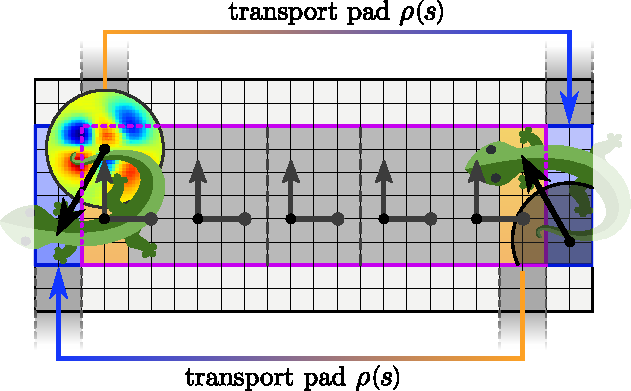
\includegraphics[width=\linewidth]{figures/mobius_conv_numerical.pdf}
	\end{subfigure}
	% new paragraph for correct alignment
	\par
	% (manually) wrapped caption, adapted from
	% https://tex.stackexchange.com/questions/158868/is-it-possible-to-let-captions-wrap-a-bit-around-includegraphics-within-figures
	% https://tex.stackexchange.com/questions/51839/wrap-caption-around-tikz-figure/51842#51842
	% The caption
	\vspace*{\dimexpr-\parskip-160.pt\relax}% Skip backwards over last left-aligned image
	\parshape 18 % Set flow of caption: N lines...
	.62\textwidth .37\textwidth % First N-1 start @ .62\textwidth with a width of .37\textwidth
	.62\textwidth .37\textwidth
	.62\textwidth .37\textwidth
	.62\textwidth .37\textwidth
	.62\textwidth .37\textwidth
	.62\textwidth .37\textwidth
	.62\textwidth .37\textwidth
	.62\textwidth .37\textwidth
	.62\textwidth .37\textwidth
	.62\textwidth .37\textwidth
	.62\textwidth .37\textwidth
	.62\textwidth .37\textwidth
	.62\textwidth .37\textwidth
	.62\textwidth .37\textwidth
	.62\textwidth .37\textwidth
	.62\textwidth .37\textwidth
	.62\textwidth .37\textwidth
	.01\textwidth .98\textwidth % the last (N-th) line flows from 0 to .99 = .62+.37 = .01+.98 ad infinitum
	\makeatletter
	\setcounter{\@captype}{\value{\@captype}-1} % \setcounter{CounterName}{number}
	\refstepcounter{\@captype}% Increase float/caption counter
	\addcontentsline{\csname ext@\@captype\endcsname}{\@captype}% Add content to "List of..."
	{\protect\numberline{\csname the\@captype\endcsname}{ورودی جدول محتویات}}%
	\small % switch to small font for caption and Figure XX:
	\csname fnum@\@captype\endcsname: % Float caption + #
	\makeatother
	% Actual caption
	نمایش عددی میدان‌های ویژگی روی نوار موبیوس و انتقال لوی-چیویتا بردارهای ویژگی در طول کانولوشن.
	هندسه مسطح نوار امکان برش و صاف کردن ایزومتریک آن را به مستطیل صورتی فراهم می‌کند.
	هنگام تخصیص چارچوب‌های مرجع کانونی $\R^2$ این امر متناظر با چسباندن دو چارت $V^A$ و $V^B$ از شکل~\ref{fig:mobius_conv_gauges} در همپوشانی آن‌ها با تبدیلات گیج بدیهی (``$\id$'') است.
	برای جلوگیری از افزونگی، ما نیمی از عرض همپوشانی چارت دوم را با تبدیلات گیج بازتابی (``$\operatorname{flip}$'') به هر انتهای نوار صاف شده صورتی (پیکسل‌های نارنجی) اختصاص می‌دهیم.
	میدان‌های ویژگی به عنوان آرایه‌ای با ابعاد فضایی متناظر با جعبه صورتی و $c$ کانال ذخیره می‌شوند.
	در طول عملیات کانولوشن، کرنل ویژگی‌ها را از تمام پیکسل‌هایی که پوشش می‌دهد جمع‌آوری می‌کند.
	با انتخاب اندازه کرنل $5\times5$ پیکسل، باید تمام مقادیر در شعاع $2$ پیکسل اطراف مرکز آن را مشخص کنیم، که به طور کلی نیاز به پد کردن نواحی مرزی $2$ پیکسل اطراف مستطیل صورتی دارد.
	مرز بالا و پایین متناظر با مرز نوار است.
	از آنجا که هیچ مقدار ویژگی معتبری نمی‌توان در آنجا تخصیص داد، آرایه را با صفر پد می‌کنیم همانطور که معمولاً در بینایی کامپیوتر انجام می‌شود.
	مرزهای چپ و راست نوار صاف شده با یک پیچ به هم چسبانده شده‌اند.
	ما انتقال موازی آن ویژگی‌ها را با برش ناحیه‌ای به عرض دو پیکسل از هر انتهای نوار (نارنجی) و پد کردن آن‌ها به صورت بازتاب یافته به انتهای مقابل (آبی) پیاده‌سازی می‌کنیم.
	همانطور که پیچ مستلزم تبدیل گیج است، میدان‌های ویژگی باید هنگام بازتاب یافتن تحت عمل $\rho(s)$ قرار گیرند.
	پس از پد کردن، کانولوشن با شرایط مرزی ``معتبر'' اجرا می‌شود، به طوری که خروجی آن دوباره اندازه جعبه صورتی را داشته باشد.
	عملیاتی که به صورت نقطه‌ای عمل می‌کنند نیاز به پد کردن ندارند اما می‌توانند بلافاصله روی آرایه صورتی اعمال شوند.
	{
		\\ \color{gray} \scriptsize
		(مارمولک‌ها تحت مجوز Creative Commons Attribution 4.0 International
		\href{https://github.com/twitter/twemoji/blob/gh-pages/LICENSE-GRAPHICS}{\underline{اقتباس شده}}
		با مجوز Twitter.)
	}
	\label{fig:mobius_conv_numerical}
\end{figure}

توجه داشته باشید که این نمایش به دلیل همپوشانی $U^A \cap U^B \neq \varnothing$ چارت‌ها افزونه است.
برای حذف این افزونگی باید آن نواحی را که دو بار نمایش داده می‌شوند شناسایی کرد و تنها یک کپی مشترک از بردارهای ویژگی متناظر را ذخیره کرد.
یک طرح ممکن برای انجام این کار، که ما در پیاده‌سازی عددی خود استفاده می‌کنیم، ذخیره میدان‌های ویژگی در آرایه چندبعدی متناظر با مستطیل صورتی در شکل~\ref{fig:mobius_conv_numerical} است.
می‌توان آن را به عنوان تعریف شده توسط ``چسباندن'' آن نواحی در $V^A$ و $V^B$ که توسط تبدیلات گیج \emph{بدیهی} $g^{BA}$ شناسایی می‌شوند در نظر گرفت (``$\id$'' در شکل~\ref{fig:mobius_conv_gauges} و چهار پیکسل مرکزی در شکل~\ref{fig:mobius_conv_numerical}).
آنچه باقی می‌ماند افزونگی بردارهای ویژگی در ناحیه همپوشانی دوم با تبدیلات گیج بازتابی است (``$\operatorname{flip}$'' در شکل~\ref{fig:mobius_conv_gauges}).
این افزونگی با تخصیص آن بردارهای ویژگی به صورت مساوی به هر انتهای نمایش میدان محلی ``چسبانده شده'' حل می‌شود (پیکسل‌های نارنجی در شکل~\ref{fig:mobius_conv_numerical}).
در مجموع، پیکسل‌های جعبه صورتی فضای ویژگی را به صورت غیرافزونه با تخصیص یک بردار ویژگی $c$-بعدی به هر یک از آنها نمایش می‌دهند.
حلقه دو پیکسلی اطراف مستطیل صورتی \emph{بخشی از} فضای ویژگی نیست بلکه ناحیه پد کردن را تجسم می‌کند که تنها در طول پاس رو به جلوی عملیات کانولوشن همانطور که در زیر بحث شده است استفاده خواهد شد.

ابعاد (شکل) واقعی آرایه‌ای که فضای ویژگی را کدگذاری می‌کند به چندگانگی‌های میدان انتخاب شده بستگی دارد.
فرض کنید $m_{\textup{triv}}$، $m_{\textup{sign}}$ و $m_{\textup{reg}}$ آن چندگانگی‌های صحیح میدان‌های ویژگی باشند که فضای ویژگی را تشکیل می‌دهند.
از آنجا که میدان‌های اسکالر و تغییر علامت یک‌بعدی هستند و میدان‌های ویژگی منظم دوبعدی هستند، تعداد کل کانال‌ها (یا بعد بردارهای ویژگی انباشته شده) توسط $c = m_{\textup{triv}} + m_{\textup{sign}} + 2 m_{\textup{reg}}$ داده می‌شود.
فرض کنید همچنین که وضوح فضایی مستطیل صورتی $X\times Y$ پیکسل باشد و اندازه دسته $N$ نمونه فرض کنید.
آرایه‌ای که فضای ویژگی را کدگذاری می‌کند سپس از شکل $(N,c,X,Y)$ است، همانطور که معمولاً در پردازش تصویر استفاده می‌شود.
توجه داشته باشید که این نمایش عددی فضای ویژگی هم نسبت به هندسه پیچیده نوار و هم نوع واقعی میدان‌های ویژگی موجود (به جز بعد آنها) بی‌اطلاع است.
بنابراین اطلاعات هندسی واقعی منحصراً توسط لایه‌های شبکه که میدان‌ها را پردازش می‌کنند حمل می‌شود.



\paragraph{جمع بایاس:}
برای پیاده‌سازی جمع بایاس مستقل از جهت‌گیری، نتایج بخش~\ref{sec:mobius_bias} را به خاطر بیاورید که فضاهای برداری بایاس‌های الگوی هم‌متغیر بازتاب برای میدان‌های اسکالر و میدان‌های منظم یک‌بعدی و برای میدان‌های تغییر علامت صفربعدی هستند.
در مقداردهی اولیه ماژول بایاس بنابراین یک بردار پارامتر $m_{\textup{triv}}$-بعدی $\beta_{\textup{triv}}$ و یک بردار پارامتر $m_{\textup{reg}}$-بعدی $\beta_{\textup{reg}}$ اختصاص می‌دهیم.
در طول پاس رو به جلو این پارامترها را به یک بردار بایاس $c$-بعدی $b_{\textup{full}}$ گسترش می‌دهیم که باید به انباشت کامل میدان‌های ویژگی اضافه شود.
این کار با اختصاص آرایه $c$-بعدی از صفرها و پر کردن $m_{\textup{triv}}$ عنصر اول با پارامترهای بایاس میدان اسکالر و $2m_{\textup{reg}}$ عنصر آخر با پارامترهای بایاس میدان منظم $m_{\textup{reg}}$، هر کدام دو بار تکرار شده برای برآوردن ساختار فضای حل در معادله~\eqref{eq:bias_solution_space_regular}، انجام می‌شود.
پس از این گسترش بردار بایاس کامل
\begin{align}
	b_{\textup{full}}\ =\ \big[
	\underbrace{
		\beta_{\textup{triv},1}, \,\dots,\, \beta_{\textup{triv}, m_{\textup{triv}}}
	}_{m_{\textup{triv}}},\ 
	\underbrace{
		0, \,\dots,\, 0,\ 
	}_{m_{\textup{sign}}},\ 
	\underbrace{
		\beta_{\textup{reg},1},\beta_{\textup{reg},1}, \,\dots,\, \beta_{\textup{reg}, m_{\textup{reg}}}, \beta_{\textup{reg}, m_{\textup{reg}}}
	}_{2m_{\textup{reg}}}
	\big]^\top \ \in\ \R^c
\end{align}
طبق معمول به آرایه میدان ویژگی اضافه می‌شود.
استقلال آن از جهت‌گیری (ناوردایی گیج) اضافه کردن به آرایه در شکل~\ref{fig:mobius_conv_numerical} را توجیه می‌کند، علی‌رغم اینکه از بردارهای ویژگی در دو گیج مختلف چسبانده شده است.



\paragraph{غیرخطی‌ها:}
غیرخطی‌ها را می‌توان مطابق تعریف در بخش~\ref{sec:mobius_nonlin} به صورت مستقیم پیاده‌سازی کرد.
این کار را با تقسیم انباشت کامل میدان‌های ویژگی به سه انباشت از میدان‌های همان نوع، اعمال غیرخطی‌های هم‌متغیر بازتاب مربوطه به آنها، و در نهایت الحاق نتایج انجام می‌دهیم.
به دلیل تعریف غیرخطی برای میدان‌های تغییر علامت در معادله~\eqref{eq:signflip_nonlin} با بایاس قابل یادگیری، ماژول غیرخطی دارای $m_{\textup{sign}}$ پارامتر قابل آموزش است.




\paragraph{کانولوشن‌های \textit{GM}:}
از آنجا که عملیات کانولوشن به صورت نقطه‌ای عمل نمی‌کنند بلکه تمام ویژگی‌های پوشش داده شده توسط کرنل را انباشت می‌کنند، پیاده‌سازی آنها کمتر بدیهی است.
پاس رو به جلو به سه گام تقسیم می‌شود، یعنی
1) گسترش کرنل‌های متقارن بازتاب از آرایه‌های پارامتر،
2) انتقال لوی-چیویتا بردارهای ویژگی و
3) کانولوشن $\GM$ واقعی.

به خاطر بیاورید که فضای $\KR$ کرنل‌های $\Flip$-هدایت‌پذیر زیرفضای خطی فضای کرنل‌های بدون قید $\mathscr{K}$ در معادله~\eqref{eq:unconstrained_kernel_space} است.
برای پارامتری کردن کرنل‌های $\Flip$-هدایت‌پذیر لازم است پایه‌ای از $\KR$ انتخاب کنیم که کرنل‌ها بر حسب آن گسترش یابند.
پارامترهای قابل آموزش عملیات کانولوشن ضرایب گسترش در این پایه هستند.
پیاده‌سازی ما تمام کرنل‌هایی را که متناظر با همان جفت انواع میدان ورودی و خروجی هستند به صورت مشترک پارامتری می‌کند
زیرا آنها تقارن‌های یکسان و بنابراین پایه یکسان دارند.
با در نظر گیری نه جفت انواع میدان نشان داده شده در جدول~\ref{tab:reflection_steerable_kernels}، این بدان معناست که ماژول کانولوشن نه آرایه پارامتر متناظر نگه می‌دارد.
کرنل‌های واقعی سپس از این پارامترها در طول هر پاس رو به جلو گسترش می‌یابند.
برای مثال، زیرمجموعه کانال‌های کرنل را در نظر بگیرید که از $m_{\textup{triv}}$ میدان اسکالر به $m_{\textup{sign}}$ میدان تغییر علامت نگاشت می‌کنند و اندازه کرنل $s\times s$ پیکسل فرض کنید.
آرایه پارامتر متناظر سپس از شکل $(m_{\textup{sign}},\, m_{\textup{triv}},\, \frac{s}{2},\, s)$ است و $m_{\textup{triv}}\times m_{\textup{sign}}$ کانال کرنل منفرد را با پایه‌ای از $\frac{s}{2}\times s$ کرنل \emph{نامتقارن} هر کدام نمایش می‌دهد.
گسترش به عنوان پر کردن $\frac{s}{2}\times s$ پیکسل بالا با پارامترهای تغییر نیافته در حالی که $\frac{s}{2}\times s$ پیکسل پایین با پارامترهای منفی شده و بازتاب یافته پر می‌شوند، پیاده‌سازی می‌شود.
به عنوان مثال دوم، کانال‌های کرنل را در نظر بگیرید که از $m_{\textup{reg}}$ میدان منظم به $m_{\textup{triv}}$ میدان اسکالر نگاشت می‌کنند.
آرایه پارامتر برای این حالت از شکل $(m_{\textup{triv}},\, m_{\textup{reg}},\, s,\, s)$ است و یکی از دو کانال کرنل به ازای هر میدان ورودی و خروجی را ذخیره می‌کند.
کانال‌های دوم متقارن در طول پاس رو به جلو با بازتاب کانال‌های کرنل اول همانطور که در جدول~\ref{tab:reflection_steerable_kernels} نشان داده شده گسترش می‌یابند.
پس از گسترش کرنل کامل به این شکل از تمام زیربلوک‌های آن متناظر با ترکیب‌های مختلف انواع میدان، شکل معمول کرنل‌ها در یادگیری عمیق را دارد اما تضمین می‌شود که تقارن‌های مشتق شده در بخش~\ref{sec:mobius_kernel_spaces} را رعایت کند.
توجه داشته باشید که تقارن‌های کرنل کانولوشن‌های $\GM$ را نسبت به \CNN غیرهم‌متغیر متناظر با همان تعداد کانال~$c$ از نظر پارامتر کارآمدتر می‌کند.
به طور خاص برای کرنل $\Flip$-هدایت‌پذیر تعداد پارامترها با ضریب دو کاهش می‌یابد%
\footnote{
	بهبود کارایی پارامتر کرنل‌های $\Flip$-هدایت‌پذیر با ضریب $2$ برای کرنل‌های پیوسته یا برای اندازه‌های کرنل زوج $s$ دقیق است.
	اگر $s$ فرد باشد، تعداد پارامترها برای کرنل‌های متقارن مثل $s(s+1)/2$ و برای کرنل‌های نامتقارن مثل $s(s-1)/2$ مقیاس می‌شود زیرا اولی ردیف مرکزی پیکسل‌ها را آزادانه پارامتری می‌کند در حالی که دومی باید آنها را روی صفر تنظیم کند.
}.


پس از گسترش کرنل‌ها، آنها با میدان‌های ویژگی کانولو می‌شوند.
این امر نیاز به پیاده‌سازی نگاشت نمایی و انتقال‌دهنده‌های لوی-چیویتا $\Flip$-سازگار روی نوار موبیوس دارد -- یا بهتر بگوییم روی نمایش عددی آن توسط آرایه صورتی از شکل~\ref{fig:mobius_conv_numerical}.
هندسه مسطح نوار موبیوس پیاده‌سازی را تقریباً بدیهی می‌کند، با این حال، مرزها و اتصال دایره‌ای آن نیاز به دقت خاصی دارند.
بنابراین باید بین سه حالت کیفی متفاوت تمایز قائل شویم که متناظر با موارد زیر هستند
1) نگاشت‌های نمایی که کاملاً در آرایه صورتی قرار دارند،
2) نگاشت‌های نمایی که از مرز عبور می‌کنند و بنابراین خوش‌تعریف نیستند و
3) نگاشت‌هایی که ژئودزیک‌هایشان از یک انتهای آرایه خارج شده و (پیچیده) از انتهای دیگر وارد می‌شوند.
حالت اول بدیهی است و متناظر با نگاشت نمایی روی خود $\R^2$ است.
از آنجا که نوار مسطح است و چارچوب‌های مرجع درون آرایه همه موازی هستند، انتقال در امتداد این ژئودزیک‌ها بدیهی است.
در ناحیه داخلی آرایه، جایی که کرنل‌های (با پشتیبانی متناهی) از آن بیرون نمی‌زنند، بنابراین می‌توان کانولوشن را طبق معمول روی $\R^2$ پیاده‌سازی کرد.
حالت دوم مربوط به ردیف‌های بالا و پایین آرایه است که در آن نگاشت‌های نمایی ممکن است از مرز نوار (یا آرایه) عبور کنند.
این شبیه مسائل مرزی برای تصاویر مسطح مستطیلی معمول است، که معمولاً با پد کردن صفر حل می‌شود.
با اتخاذ این راه‌حل، آرایه را با ردیف‌هایی از صفر پد می‌کنیم که به عنوان دو نوار خاکستری روشن بالا و پایین مستطیل صورتی در شکل~\ref{fig:mobius_conv_numerical} نشان داده شده‌اند.
با اندازه کرنل $s\times s$ پیکسل با $s$ فرد، باید $(s-1)/2$ ردیف صفر در هر دو طرف پد کرد.
حالت سوم در انتهای چپ و راست آرایه رخ می‌دهد، جایی که نوار برای صاف کردن بریده شده است.
شکل~\ref{fig:mobius_conv_numerical} ژئودزیک نمونه‌ای را تجسم می‌کند که از خط برش عبور می‌کند و بنابراین در جهت بازتاب یافته از طرف مقابل وارد آرایه می‌شود.
به دلیل بازتاب، انتقال‌دهنده موازی در سراسر برش توسط $\rho(s)$ داده می‌شود.
برای اینکه بتوانیم روتین کانولوشن متعارف اجرا کنیم، انتقال در سراسر برش را با کپی کردن ناحیه $(s-1)/2$ پیکسل از هر دو انتهای آرایه (نارنجی)، بازتاب آنها به صورت وارونه برای مدل‌سازی پیچ، عمل روی آنها با $\rho(s)$ برای در نظر گیری گیج‌های بازتاب یافته و در نهایت الحاق آنها به طرف مقابل آرایه (آبی) پیاده‌سازی می‌کنیم.
با پد کردن آرایه به این شکل، تمام ژئودزیک‌ها و انتقال‌دهنده‌های مربوطه به همتایان بدیهی خود روی $\R^2$ کاهش می‌یابند.

به طور کلی، پیاده‌سازی ما از عملیات کانولوشن سه گام فوق‌الذکر را اعمال می‌کند.
ابتدا کرنل‌های $\Flip$-هدایت‌پذیر را گسترش می‌دهد و آرایه میدان ویژگی صورتی را با صفرها و مقادیر میدان که در سراسر برش منتقل می‌شوند پد می‌کند.
کرنل گسترش یافته سپس با میدان‌های ویژگی پد شده کانولو می‌شود و روتین کانولوشن متعارف برای تصاویر مسطح فراخوانی می‌شود.
ما تنظیمات مرزی ``معتبر'' برای کانولوشن استفاده می‌کنیم، که به این معناست که عملیات به طور ضمنی صفرهای بیشتری پد نمی‌کند و تنها بردارهای ویژگی را برای آن نقاطی محاسبه می‌کند که کرنل از مرزهای آرایه دستی پد شده ما فراتر نمی‌رود.
میدان ویژگی حاصل بنابراین دوباره همان ابعاد فضایی مستطیل صورتی اصلی را خواهد داشت.




\paragraph{\lr{Pooling}:}
\lr{CNN}های متعارف معمولاً عملیات \lr{pooling} فضایی را اعمال می‌کنند که بردارهای ویژگی از یک پنجره \lr{pooling} داده شده، به عنوان مثال ناحیه‌ای از پیکسل‌های $2\times2$، را در یک بردار ویژگی جدید خلاصه می‌کنند.
چنین عملیاتی وضوح فضایی را کاهش می‌دهد که هزینه محاسباتی را کاهش داده و میدان دید مؤثر کرنل‌های کانولوشن را افزایش می‌دهد.
روش رایج \lr{pooling} به اصطلاح \lr{``max-pooling''} است که بیشترین مقدار هر کانال ویژگی فردی در ناحیه \lr{pooling} را انتخاب می‌کند.
این عملیات را می‌توان مستقیماً روی میدان‌های اسکالر اعمال کرد زیرا آنها ناوردای پیمانه هستند.
همچنین برای میدان‌های ویژگی منتظم قابل قبول است زیرا گرفتن بیشینه با جابجایی کانال‌ها جابجا می‌شود.
با این حال، از آنجا که میدان‌های \lr{sign-flip} علامت خود را تحت تبدیلات پیمانه تغییر می‌دهند، \lr{max-pooling} نسبت به قانون تبدیل آنها هموردا نیست.
جایگزین هموردا، \lr{average pooling} است که میانگین ویژگی‌ها در ناحیه \lr{pooling} را می‌گیرد و بنابراین با تغییر علامت جابجا می‌شود.
گزینه دیگر، که در آزمایش‌های زیر استفاده می‌کنیم زیرا کمی بهتر عمل می‌کند، این است که میدان‌های \lr{sign-flip} را بر اساس قدر مطلق آنها \lr{pool} کنیم که مجدداً تحت وارونگی علامت ناوردا است.
سپس علامت مقادیر میدان \lr{pool} شده را با بیشترین نُرم ضرب می‌کنیم تا قانون تبدیل اصلی حفظ شود.

در حالی که عملیات \lr{pooling} تعریف شده به این شکل نسبت به تبدیلات پیمانه هموردا هستند، اصل طراحی آنها اساساً با هموردایی ایزومتری مطلوب تداخل دارد.
این بدان دلیل است که آنها وضوح فضایی گسسته‌سازی عددی را کاهش می‌دهند، به طوری که خروجی تنها نسبت به زیرگروه تقارن‌های شبکه با وضوح پایین‌تر دقیقاً هموردا است.
این اثر برای \lr{CNN}های متعارف به خوبی شناخته شده است~\cite{azulay2018shift}.
اگرچه تلاش‌هایی برای اصلاح وضعیت انجام شده~\cite{zhang2019CNNsShiftInvariant}، از دست رفتن جزئی هموردایی انتقالی (یا ایزومتری) به یک زیرگروه معمولاً همانطور که هست پذیرفته می‌شود.

\paragraph{تست‌های واحد:}
تمام عملیات مستقل از مختصات پیشنهادی برای تضمین هموردایی پیمانه و هموردایی ایزومتری آنها تست واحد می‌شوند.
تست‌های هموردایی پیمانه برای تمام عملیات پیشنهادی و همچنین برای کل شبکه‌های توصیف شده در بخش بعدی موفق هستند.
برای کانولوشن، جمع \lr{bias} و غیرخطی‌ها، تست‌های واحد ما تأیید می‌کنند که هموردایی ایزومتری دقیقاً برقرار است.
همانطور که انتظار می‌رود، عملیات \lr{pooling} فضایی نسبت به تقارن‌های شبکه با وضوح بالا دقیقاً هموردا نیستند.%
\footnote{
	توجه کنید که این مسئله برای عملیات \lr{pooling} ذاتی است و برای \lr{CNN}های متعارف نیز صدق می‌کند~\cite{azulay2018shift,zhang2019CNNsShiftInvariant}.
}
با این حال، هموردایی ایزومتری آنها را برای آن زیرگروه از ایزومتری‌ها که همزمان تقارنی از شبکه با وضوح پایین‌تر هستند تأیید می‌کنیم.
نتایج تجربی ما، که در ادامه بحث می‌کنیم، نشان می‌دهند که هموردایی ایزومتری غیردقیق، ناوردایی ایزومتری پیش‌بینی‌های طبقه‌بندی یک شبکه کامل را در اکثر موارد تنها به طور حاشیه‌ای تحت تأثیر قرار می‌دهد.

\subsubsection{ارزیابی تجربی}
\label{sec:mobius_evaluation}

عملیات مستقل از مختصات و ویژگی‌های هموردایی ادعا شده آنها را روی یک وظیفه طبقه‌بندی ساده تصاویر \lr{MNIST} که روی نوار مؤبیوس پروژکت شده‌اند، ارزیابی می‌کنیم.
ترکیبات مختلف انواع میدان با نمونه‌سازی معماری‌های مدل مشابه برای آنها مقایسه می‌شوند.
به عنوان خط مبنا، یک \lr{CNN} غیرمستقل از مختصات را روی نوار مؤبیوس آموزش می‌دهیم که به طور قابل توجهی توسط مدل‌های هموردا بهتر عمل می‌کند.

مجموعه داده \lr{M\"obius MNIST} با گرفتن ارقام استاندارد \lr{MNIST} $28\times28$ پیکسل و پروژکت کردن آنها روی نوار با شناسایی مرز چپ و راست با یک پیچش اضافی ساخته می‌شود.
مطابق با مجموعه داده \lr{MNIST} چرخانده شده، که یک معیار استاندارد برای \lr{CNN}های اقلیدسی هموردای دورانی است، اندازه مجموعه آموزش را به $12000$ نمونه کاهش می‌دهیم~\cite{Weiler2018SFCNN,Weiler2019_E2CNN}.
از آنجا که \lr{MNIST} شامل ارقام خاکستری تک کاناله است که تحت تبدیلات پیمانه ناوردا هستند، نمونه‌های آن به عنوان میدان‌های اسکالر شناسایی می‌شوند.
بنابراین هر نمونه با آرایه‌ای به شکل $(1,28,28)$ نمایش داده می‌شود که متناظر با مستطیل بنفش در شکل~\ref{fig:mobius_conv_numerical} است.
توجه کنید که شناسایی مرز چپ و راست برای مورد خاص ارقام \lr{MNIST} منجر به هیچ ناپیوستگی نمی‌شود زیرا رنگ پس‌زمینه آنها سیاه ثابت (یعنی صفر) است.
به منظور نمایش هموردایی ایزومتری القا شده \lr{CNN}های مستقل از مختصات، دو نسخه از این مجموعه داده می‌سازیم.
اولی شامل ارقامی است که همگی \emph{متمرکز} هستند، یعنی در همان موقعیت روی نوار قرار دارند.
مجموعه داده دوم ارقام را در موقعیت‌های تصادفی اطراف نوار قرار می‌دهد، یعنی آنها را با ایزومتری‌های نمونه‌برداری تصادفی \emph{جابجا} می‌کند همانطور که در شکل~\ref{fig:mobius_conv_isometries} تجسم شده است.
انتظار می‌رود هر مدل هموردای ایزومتری استنتاج خود را از مجموعه داده ارقام متمرکز به مجموعه داده جابجا شده ایزومتری تعمیم دهد که توسط آزمایش‌های ما تأیید می‌شود.
در حالی که \lr{M\"obius MNIST} به وضوح یک مجموعه داده اسباب‌بازی است، تمام ویژگی‌های نظری که ما به آنها علاقه‌مندیم را نشان می‌دهد و به عنوان یک مورد تست راحت برای نمایش تفاوت بین \lr{CNN}های متعارف و \lr{CNN}های مستقل از مختصات عمل می‌کند.

تمام معماری‌های شبکه همانطور که معمول است به عنوان یک سری لایه‌های کانولوشنی، که با یک عملیات \lr{pooling} سراسری و یک طبقه‌بندی‌کننده ناوردا و کاملاً متصل دنبال می‌شوند، ساخته می‌شوند؛ جدول~\ref{tab:mobius_model_architectures} را برای مقایسه ببینید.
بخش‌های کانولوشنی از شش بلوک کانولوشنی با عملیات \lr{pooling} فضایی پس از بلوک کانولوشن دوم و چهارم ساخته می‌شوند.
بلوک‌های کانولوشن کاملاً اساسی هستند و تنها از یک لایه کانولوشنی که با جمع \lr{bias} و یک لایه غیرخطی دنبال می‌شود تشکیل شده‌اند.
تمام عملیات \lr{pooling} میانی از پنجره‌های \lr{pooling} $2\times2$ پیکسل استفاده کرده و بنابراین وضوح فضایی را نصف می‌کنند.
در مورد مدل‌های هموردای بازتاب، آخرین لایه کانولوشنی به $64$ میدان اسکالر نقشه می‌برد.
ناوردایی آنها تحت تبدیلات پیمانه تضمین می‌کند که عملیات \lr{global max-pooling} بعدی ویژگی‌های \emph{هم ناوردای موقعیت و هم ناوردای پیمانه} تولید کند.
یک \lr{MLP} با فعال‌سازی \lr{softmax} نهایی آن ویژگی‌ها را برای تولید پیش‌بینی‌های ناوردا می‌گیرد.
برای تمام مدل‌ها از همان دو بلوک \lr{MLP} تشکیل شده است که \lr{batch-normalization}، غیرخطی \lr{ELU}، \lr{dropout} با احتمال حذف $30\%$ و یک لایه خطی (یا \lr{affine}) اعمال می‌کنند که تعداد نورون‌های خروجی آن در جدول~\ref{tab:mobius_model_architectures} فهرست شده است.
بنابراین تفاوت‌های بین مدل‌های مختلف به بخش کانولوشنی محدود می‌شود.

\begin{table}
	\centering
	\footnotesize
	\setlength{\tabcolsep}{8pt}
	\begin{tabular}{lccccccc}
		\toprule
		لایه              & \multicolumn{6}{c}{چندگانگی میدان‌های خروجی $(m_{\textup{triv}},m_{\textup{sign}},m_{\textup{reg}})$ / کانال‌ها / نورون‌ها}   \\
		& اسکالر        & \lr{sign-flip}     & منتظم       & \lr{irreps}          & مختلط          & \lr{CNN} \\[.25ex]
		\midrule
		ورودی شبکه      &  $( 1, 0, 0)$ &  $(1,  0, 0)$ & $(1, 0,  0)$  &  $(1,  0, 0)$   &    $(1, 0, 0)$ & $1$ \\
		بلوک کانولوشن         &  $(16, 0, 0)$ &  $(0, 16, 0)$ & $(0, 0,  8)$  &  $(8,  8, 0)$   &    $(4, 4, 2)$ & $\lfloor 16/\sqrt{\alpha}\rfloor$ \\
		بلوک کانولوشن         &  $(32, 0, 0)$ &  $(0, 32, 0)$ & $(0, 0, 16)$  & $(16, 16, 0)$   &    $(8, 8, 4)$ & $\lfloor 32/\sqrt{\alpha}\rfloor$ \\
		\lr{pooling}            & همان        & همان        & همان        & همان          & همان         & همان                            \\
		بلوک کانولوشن         &  $(64, 0, 0)$ &  $(0, 64, 0)$ & $(0, 0, 32)$  & $(32, 32, 0)$   & $(16, 16,  8)$ & $\lfloor 64/\sqrt{\alpha}\rfloor$ \\
		بلوک کانولوشن         & $(128, 0, 0)$ & $(0, 128, 0)$ & $(0, 0, 64)$  & $(64, 64, 0)$   & $(32, 32, 16)$ & $\lfloor128/\sqrt{\alpha}\rfloor$ \\
		\lr{pooling}            & همان        & همان        & همان        & همان          & همان         & همان                            \\
		بلوک کانولوشن         & $(256, 0, 0)$ & $(0, 256, 0)$ & $(0, 0, 128)$ & $(128, 128, 0)$ & $(64, 64, 32)$ & $\lfloor256/\sqrt{\alpha}\rfloor$ \\
		بلوک کانولوشن         &  $(64, 0, 0)$ &  $(64, 0, 0)$ &  $(64, 0, 0)$ & $(64, 0, 0)$    & $(64, 0, 0)$   & $64$                              \\
		\midrule
		\lr{global max-pooling} & $64$          & $64$          & $64$          & $64$            & $64$           & $64$           \\
		بلوک \lr{MLP}          & $32$          & $32$          & $32$          & $32$            & $32$           & $32$           \\
		بلوک \lr{MLP} + \lr{softmax} \hspace*{-3ex}
		& $10$          & $10$          & $10$          & $10$            & $10$           & $10$           \\
		\bottomrule
	\end{tabular}
	%%%%%%%%%%%%%%%%%%%%%%%%%%%%%%%%%%%%%%%%%%%%%%%%%%%%%%%%%%%%%%%%%%%%%%%%%%%%%%%%%%%%%%%%%%%%%%%%%%%%%%%%%%%%%%%%%%%%%%%%%%%%%
	\vspace*{2.ex}
	\caption[]{\small
		نمای کلی معماری‌های مدل مقایسه شده.
		تمام مدل‌ها از یک بخش کانولوشنی روی نوار مؤبیوس، که با یک عملیات \lr{global max-pooling} و یک طبقه‌بندی‌کننده \lr{MLP} دنبال می‌شود، تشکیل شده‌اند.
		پنج \lr{CNN} مستقل از جهت‌گیری در چندگانگی‌های $(m_{\textup{triv}},m_{\textup{sign}},m_{\textup{reg}})$ انواع میدان متفاوت هستند اما دقیقاً در تعداد کانال‌ها و تقریباً در تعداد پارامترها موافق هستند.
		ورودی‌های آنها، یعنی ارقام \lr{MNIST}، به عنوان میدان‌های اسکالر فرض می‌شوند.
		تمام مدل‌های مستقل از جهت‌گیری در آخرین کانولوشن خود به $64$ میدان اسکالر ناوردای پیمانه نقشه می‌برند.
		عملیات \lr{pooling} سراسری بعدی بنابراین ویژگی‌های ناوردای موقعیت و مستقل از مختصات تولید می‌کند.
		مدل \lr{CNN} خط مبنا در دو نوع ارائه می‌شود که در ضریب $\sqrt{\alpha}$ آنها در تعداد کانال‌ها متفاوت هستند.
		نسخه اول $\alpha=1$ فرض کرده و بنابراین همان تعداد کانال مدل‌های مستقل از مختصات را استفاده می‌کند.
		به دلیل کارایی پارامتر پایین‌تر \lr{CNN}های غیرهموردا، این مدل تقریباً دو برابر پارامتر بیشتری استفاده می‌کند.
		برای مقایسه عادلانه نسخه دومی با $\alpha=2$ و بنابراین تقریباً همان تعداد پارامتر مدل‌های هموردا اضافه می‌کنیم.
	}
	\label{tab:mobius_model_architectures}
\end{table}

پنج مدل مستقل از مختصاتی که نمونه‌سازی می‌کنیم در انواع میدان استفاده شده متفاوت هستند:
سه مدل خالص وجود دارد که با \lr{``scalar''}، \lr{``sign-flip''} و \lr{``regular''} نشان داده می‌شوند که تنها نوع میدان پیشنهادی را فرض می‌کنند.
به دلیل بُعد بالاتر، چندگانگی‌های میدان میدان‌های ویژگی منتظم در مقایسه با میدان‌های اسکالر و \lr{sign-flip} نصف می‌شوند.
مدل چهارم، که با \lr{``irrep''} نشان داده می‌شود، از ترکیبی از میدان‌های اسکالر و \lr{sign-flip} به نسبت‌های مساوی استفاده می‌کند.
توجه کنید که میدان‌های ویژگی این مدل به صورت خطی معادل مدل‌های \lr{``regular''} هستند زیرا تغییر پایه از معادله~\eqref{eq:rho_reg_decomposition} بین هر دو ترجمه می‌کند.
مدل پنجم، \lr{``mixed''} هر سه نوع میدان را اعمال می‌کند.
غیرخطی‌های مورد استفاده برای انواع میدان‌های مختلف همان‌هایی هستند که در بخش~\ref{sec:mobius_nonlin} توضیح داده شده‌اند.
همانطور که قبلاً بیان شد، تمام مدل‌ها ورودی‌ها و خروجی‌های اسکالر فرض می‌کنند.

تمام لایه‌های مستقل از مختصات تست واحد شده و کاملاً هموردای پیمانه یافت شده‌اند که نشان می‌دهد مدل‌ها به طور کلی کاملاً ناوردای پیمانه هستند.
از آنجا که دو مرحله \lr{pooling} اعمال می‌کنند که وضوح فضایی را هر یک با ضریب $2$ قبل از \lr{pooling} سراسری کاهش می‌دهند، هموردایی ایزومتری (ناوردایی) تنها برای زیرگروه جابجایی‌ها به مضارب $4$ پیکسل برقرار است.
بنابراین ویژگی‌های ادعا شده نظری همانطور که انتظار می‌رود برقرار هستند.

به عنوان خط مبنا، مدل‌های هموردای بازتاب را با \lr{CNN}های متعارف وابسته به مختصات روی نوار مؤبیوس مقایسه می‌کنیم.
به منظور احترام به توپولوژی نوار، نسخه ساده‌ای از عملیات \lr{padding} انتقالی را اعمال می‌کنیم.
از آنجا که \lr{CNN}ها نسبت به انواع میدان ناآگاه هستند، این کار با گرفتن نوارهای نارنجی دو پیکسل از شکل~\ref{fig:mobius_conv_numerical} و \lr{pad} کردن آنها به طرف مقابل آرایه پس از اعمال بازتاب اما بدون عمل کردن با نمایش گروهی نامشخص انجام می‌شود -- به طور رسمی، این متناظر با انتقال ویژگی‌ها طبق یک اتصال بدیهی است.
از آنجا که عملیات غیرهموردا از نظر پارامتر کمتر کارآمد هستند، دو نسخه مختلف در نظر می‌گیریم:
نسخه اول همان تعداد \emph{کانال} مدل‌های مستقل از مختصات را استفاده می‌کند و بنابراین تقریباً دو برابر پارامتر بیشتری نیاز دارد.
تعداد کانال‌های نسخه دوم با ضریب $\sqrt{2}$ کاهش می‌یابد تا تعداد \emph{پارامترها} تقریباً معادل مدل‌های مستقل از جهت‌گیری باشد.

تمام مدل‌ها برای $20$ \lr{epoch} با اندازه \lr{batch} $128$ نمونه، کاهش وزن $10^{-6}$ و استفاده از بهینه‌ساز \lr{Adam}~\cite{Kingma2015-yq} آموزش داده می‌شوند.
نرخ یادگیری اولیه $5\cdot10^{-3}$ تا حد امکان بالا انتخاب شده بدون اینکه منجر به واگرایی فرآیند آموزش شود.
یک برنامه کاهش نرخ یادگیری ثابت اندازه گام را هر $4$ \lr{epoch} با ضریب $2$ کاهش می‌دهد.

\begin{table}
	\centering
	\renewcommand\arraystretch{1.1}
	\setlength{\tabcolsep}{12pt} % default 6pt
	\small
	\begin{tabular}{lc@{\hspace{6pt}}c@{\hspace{6pt}}crc@{\hspace{8pt}}c}
		\toprule
		مدل                   & \multicolumn{3}{c}{انواع میدان $\rho_i$}    & پارامترها        & \multicolumn{2}{c}{خطای تست (\%)}                                              \\
		& بدیهی & \lr{sign-flip} & منتظم               &               & ارقام آموزش جابجا شده               & ارقام آموزش متمرکز                       \\[.25ex]
		\midrule
		\lr{CNN (channels)}          &         & ---       &                       & $1501$\,\lr{k}    & $1{.}97 \scriptstyle\,\pm\, 0{.}11$    & $42{.}99 \scriptstyle\,\pm\, 2{.}65$ \\
		\lr{CNN (params)}            &         & ---       &                       & $832$\,\lr{k}     & $2{.}08 \scriptstyle\,\pm\, 0{.}10$    & $43{.}68 \scriptstyle\,\pm\, 2{.}85$ \\
		\lr{gauge CNN (scalar)}      & $\checkmark$  & $\times$ & $\times$     & $902$\,\lr{k}     & $1{.}60 \scriptstyle\,\pm\, 0{.}10$    & $\phantom{4} 1{.}60 \scriptstyle\,\pm\, 0{.}09$ \\
		\lr{gauge CNN (sign-flip)}   & $\times$ & $\checkmark$  & $\times$     & $820$\,\lr{k}     & $4{.}27 \scriptstyle\,\pm\, 0{.}24$    & $\phantom{4} 4{.}89 \scriptstyle\,\pm\, 0{.}36$ \\
		\lr{gauge CNN (regular)}     & $\times$ & $\times$ & $\checkmark$      & $752$\,\lr{k}     & $1{.}24 \scriptstyle\,\pm\, 0{.}08$    & $\phantom{4} 1{.}23 \scriptstyle\,\pm\, 0{.}07$ \\
		\lr{gauge CNN (irreps)}      & $\checkmark$  & $\checkmark$  & $\times$     & $752$\,\lr{k}     & $1{.}65 \scriptstyle\,\pm\, 0{.}09$    & $\phantom{4} 1{.}64 \scriptstyle\,\pm\, 0{.}12$ \\
		\lr{gauge CNN (mixed)}       & $\checkmark$  & $\checkmark$  & $\checkmark$      & $752$\,\lr{k}     & $1{.}43 \scriptstyle\,\pm\, 0{.}09$    & $\phantom{4} 1{.}42 \scriptstyle\,\pm\, 0{.}10$ \\[.25ex]
		\bottomrule
	\end{tabular}
	\vspace*{2ex}
	\caption{
		خطاهای تست معماری‌های مختلف شبکه، هر کدام میانگین‌گیری شده روی $32$ اجرا.
		ستون \lr{``shifted train digits''} عملکرد برای تنظیمی را گزارش می‌کند که در آن هم نمونه‌های آموزش و هم تست در مکان‌های تصادفی روی نوار قرار داده شده‌اند.
		در حالی که \lr{CNN}های متعارف $\RM$-مستقل از مختصات نیستند، قادر به یادگیری تشخیص ارقام همانطور که از میدان چارچوب ناپیوسته آنها دیده می‌شود هستند.
		تقریباً تمام \lr{CNN}های مستقل از مختصات نتایج بهتری به طور قابل توجهی به دست می‌آورند.
		عملکرد پایین‌تر مدل \lr{sign-flip} نشان می‌دهد که \lr{CNN}های مستقل از مختصات ممکن است زمانی که انتخاب‌های بدی از انواع میدان یا غیرخطی‌ها انجام شود خیلی خوب کار نکنند.
		ارقام آموزش در ستون \lr{``centered train digits''} همگی در همان موقعیت روی نوار قرار داده شده‌اند در حالی که ارقام تست به طور تصادفی جابجا شده باقی می‌مانند.
		\lr{CNN}های مستقل از مختصات قادر به تعمیم استنتاج خود بین هر دو وضعیت هستند که هموردایی ایزومتری آنها را تأیید می‌کند.
		در تضاد، عملکرد \lr{CNN}های متعارف بدتر می‌شود که نشان‌دهنده فقدان هموردایی آنها تحت ایزومتری‌ها است.
	}
	\label{tab:mobius_mnist_results}
\end{table}

جدول~\ref{tab:mobius_mnist_results} خطاهای تست حاصل از تمام مدل‌ها را نشان می‌دهد که هر کدام روی $32$ اجرا میانگین‌گیری شده‌اند.
تنظیم اول، که در ستون \lr{``shifted train digits''} گزارش شده، از ارقام قرار داده شده تصادفی هم در مجموعه داده آموزش و هم تست استفاده می‌کند.
هر دو نسخه \lr{CNN} غیرهموردا تقریباً همان خطای تست را به دست می‌آورند.
در تضاد، اکثر \lr{CNN}های مستقل از مختصات نتیجه بهتری به طور قابل توجهی به دست می‌آورند.
تنها مدلی که کاملاً بر میدان‌های \lr{sign-flip} مبتنی است بدتر عمل می‌کند -- این نشان می‌دهد که ترکیب استفاده شده از میدان‌های \lr{sign-flip} و غیرخطی‌ها انتخاب خوبی نیست، علی‌رغم اینکه مستقل از مختصات است.
بنابراین انتخاب‌های بد میدان‌های ویژگی و غیرخطی‌ها دیده می‌شود که به عملکرد مدل آسیب می‌زنند.
مدلی که بهترین نتایج را به دست می‌آورد بر میدان‌های ویژگی منتظم مبتنی است.
این مشاهده با یافته‌های قبلی، به عنوان مثال مقایسه سیستماتیک انواع میدان در~\cite{Weiler2019_E2CNN} همسو است.
تفسیر ما از این نتیجه این است که قیدهای کرنل شامل میدان‌های ویژگی منتظم اساساً اجازه کانال‌های کرنل بدون قید را می‌دهند، با شرط اضافی اعمال دو کپی بازتاب یافته از آنها -- این را در تضاد با کرنل‌های $\Flip$-راهبری‌پذیر بین میدان‌های \lr{irrep} ببینید که باید \emph{درون} یک کانال کرنل متقارن باشند.
مدل مبتنی بر میدان‌های اسکالر عملکرد میانی بین \lr{CNN}های متعارف و مدل میدان منتظم به دست می‌آورد.
هر دو مدلی که از انواع میدان مختلط استفاده می‌کنند عملکردی بین انواع میدان ترکیب دارند.
می‌خواهیم مجدداً تأکید کنیم که مدل منتظم و مدل \lr{irrep} دقیقاً شامل همان انواع میدان \lr{irrep} هستند اما در پایه متفاوتی بیان شده‌اند.
از آنجا که این تغییر پایه می‌تواند به عنوان بخشی از غیرخطی‌های اعمال شده تفسیر شود، این نتیجه نشان می‌دهد که غیرخطی‌های استفاده شده تأثیر عمده‌ای روی عملکرد مدل دارند.
علی‌رغم اینکه در~\cite{Weiler2019_E2CNN} بررسی شده، منظره غیرخطی‌های هموردا هنوز تا حد زیادی قلمرو ناکشف شده‌ای است.

تنظیم آموزش دوم، که در ستون \lr{``centered train digits''} گزارش شده، قابلیت مدل‌ها برای تعمیم روی تمام حالت‌هایی که توسط ایزومتری‌ها مرتبط هستند را بررسی می‌کند.
تمام مدل‌ها روی ارقامی که در همان مکان روی نوار رخ می‌دهند آموزش داده می‌شوند اما روی ارقام جابجا شده تصادفی تست می‌شوند.
همانطور که انتظار می‌رود، عملکرد \lr{CNN}های متعارف در این تنظیم به طور قابل توجهی بدتر می‌شود -- این نشان می‌دهد که آنها واقعاً تحت ایزومتری‌های نوار مؤبیوس هموردا نیستند.
در تضاد، عملکرد اکثر \lr{CNN}های مستقل از مختصات در انحراف معیار بدون تغییر باقی می‌ماند.
علی‌رغم اینکه تنها نسبت به زیرگروه ایزومتری‌هایی که به مضارب $4$ پیکسل جابجا می‌شوند دقیقاً هموردا (ناوردا) هستند، ناوردایی ایزومتری کامل مدل‌ها بنابراین به نظر خیلی خوب برقرار است.
در حالی که مدل \lr{sign-flip} در مقایسه با تنظیم آموزش اول بطور قابل توجهی بدتر می‌شود، هنوز تقریباً هموردای ایزومتری است و بنابراین خیلی بهتر از \lr{CNN}های متعارف عمل می‌کند.

در نتیجه، آزمایش‌های انجام شده ویژگی‌های ادعا شده \lr{CNN}های مستقل از مختصات را تأیید کرده و برتری آنها نسبت به مدل‌های وابسته به مختصات را نشان می‌دهند.